\chap{HÀM SỐ VÀ ĐỒ THỊ}
\setcounter{section}{0}
\section{Hàm số}

\subsection{Tóm tắt lý thuyết}
\subsubsection{Hàm số và tập xác định của hàm số}
\begin{dn}{}
	Giả sử $x$ và $y$ là hai đại lượng biến thiên và $x$ nhận giá trị thuộc tập số $\mathscr{D}$.\\
	Nếu với mỗi giá trị của $x$ thuộc tập $\mathscr{D}$, ta xác định được một và chỉ một giá trị tương ứng $y$ thuộc tập số thực $\mathbb{R}$ thì ta có một \textbf{hàm số}. \\
	Ta gọi $x$ là \textbf{biến số} và $y$ là \textbf{hàm số} của $x$.\\
	Tập hợp $\mathscr{D}$ được gọi là \textbf{tập xác định} của hàm số.\\
	Tập hợp $T$ gồm tất cả các giá trị $y$ (tương ứng với $x$ thuộc $\mathscr{D}$) được gọi là \textbf{tập giá trị} của hàm số.
\end{dn}

\subsubsection{Cách cho hàm số}

\begin{listEX}[3]
	\item Cho bằng bảng
	\item Cho bằng biểu đồ
	\item Cho bằng công thức
\end{listEX}

\begin{note}
	Khi cho hàm số bằng công thức mà không chỉ rõ tập xác định của nó thì ta quy ước \textbf{tập xác định} của hàm số $y=f(x)$ là tập hợp tất cả các số thực $x$ để biểu thức $f(x)$ \textbf{có nghĩa}.
\end{note}

\subsubsection{Đồ thị của hàm số}
\begin{dn}{}
	Cho hàm số $y=f(x)$ có tập xác định $\mathscr{D}$. Trên mặt phẳng tọa độ $Oxy$, \textbf{đồ thị} $(C)$ của hàm số là tập hợp tất cả các điểm $M(x;y)$ với $x\in\mathscr{D}$ và $y=f(x)$.\\
	Vậy $(C)=\{M(x;f(x))\mid x\in\mathscr{D}\}$.
\end{dn}

Ta thường gặp trường hợp đồ thị của hàm số $y=f(x)$ là một đường (đường thẳng, đường cong,...). Khi đó, ta nói $y=f(x)$ là \textbf{phương trình} của đường đó.

\subsubsection{Sự biến thiên của hàm số}

\begin{dn}{}
	Hàm số $y=f(x)$ gọi là \textbf{đồng biến (tăng)} trên khoảng $(a;b)$ nếu
	$$\forall x_1, x_2\in (a;b), x_1 < x_2 \Rightarrow f(x_1) < f(x_2).$$
	Hàm số $y=f(x)$ gọi là \textbf{nghịch biến (giảm)} trên khoảng $(a;b)$ nếu
	$$\forall x_1, x_2\in (a;b), x_1 < x_2 \Rightarrow f(x_1) > f(x_2).$$
\end{dn}

%\begin{note}
%	\textbf{Xét chiều biến thiên của một hàm số} là tìm các khoảng đồng biến và các khoảng nghịch biến của hàm số đó.
%\end{note} 

\begin{note}
	Khi hàm số đồng biến trên $(a;b)$ thì đồ thị của nó có dạng đi lên từ trái sang phải.\\
	Khi hàm số nghịch biến trên $(a;b)$ thì đồ thị của nó có dạng đi xuống từ trái sang phải.
\end{note}
\begin{center}
	\begin{tikzpicture}[line cap=round, line join=round, scale=.6]
		\begin{axis}[
				legend pos=outer north east,
				xlabel = $x$,
				ylabel = $y$,
				axis lines = middle
			]
			\addplot [
				domain=-2:2,
				samples=100,
				%color=blue,
			]
			{-x^2+1.5};
			% \addlegendentry{$f(x)$}
		\end{axis}
	\end{tikzpicture}
	\begin{tikzpicture}[line join = round, line cap = round,>=stealth,font=\footnotesize,scale=1]
		\tkzTabInit[nocadre=false,lgt=1.2,espcl=2.5,deltacl=0.6]
		{$x$ /0.6, $f(x)$ /2}
		{$-\infty$,$0$,$+\infty$}
		\tkzTabVar{-/$ $,+/$ $,-/$ $}
	\end{tikzpicture}
\end{center}
\subsection{Các dạng toán}

\begin{dang}{Tập xác định, tập giá trị của hàm số}
\end{dang}

\viduminhhoa

\begin{vd}%[Thành Đức Trung]%[0D2B1-2]
	Tìm tập xác định của các hàm số sau
	\begin{enumerate}
		\begin{minipage}{0.5\linewidth}
			\item $y=\dfrac{\sqrt[3]{x^2-1}}{x^2+2x+3}$.
		\end{minipage} \begin{minipage}{0.5\linewidth}
			\item $y=\dfrac{x}{x-\sqrt{x}-6}$.
		\end{minipage}
		\begin{minipage}{0.5\linewidth}
			\item $y=\sqrt{x+2}-\sqrt{x+3}$.
		\end{minipage} \begin{minipage}{0.5\linewidth}
			\item $y=\heva{ & \dfrac{1}{x} & & \text{khi} \ x\geqslant1 \\ & \sqrt{1-x} & & \text{khi} \ x<0.}$
		\end{minipage}
	\end{enumerate}
	\loigiai{
		\begin{enumerate}
			\item Điều kiện xác định $x^2+2x+3\neq0$ đúng với mọi $x$. \\
			      Vậy tập xác định của hàm số là $\mathscr{D}=\mathbb{R}$.
			\item Điều kiện xác định $\heva{ & x\geqslant0 \\ & x-\sqrt x-6\neq0} \Leftrightarrow \heva{ & x\geqslant0 \\ &\sqrt{x}\neq-2 \\ &\sqrt{x}\neq3} \Leftrightarrow \heva{ & x\geqslant0 \\ & x \neq9.}$\\
			      Vậy tập xác định của hàm số là $\mathscr{D}=[0;+\infty)\setminus\{9\}$.
			\item Điều kiện xác định $\heva{ & x+2\geqslant0 \\ & x+3\geqslant0} \Leftrightarrow \heva{ & x\geqslant-2 \\ & x\geqslant-3} \Leftrightarrow x\geqslant-2$. \\
			      Vậy tập xác định của hàm số là $\mathscr{D}=[-2;+\infty)$.
			\item Khi $x\geqslant1$ thì hàm số là $y=\dfrac{1}{x}$ luôn xác định với $x\geqslant1$. \\
			      Khi $x<0$ thì hàm số là $y=\sqrt{1-x}$ luôn xác định với $x<0$. \\
			      Vậy tập xác định của hàm số là $\mathscr{D}=(-\infty;0)\cup[1;+\infty)$.
		\end{enumerate}
	}
\end{vd}

\begin{vd}%[Thành Đức Trung]%[0D1Y1-2]
	Cho bảng giá trị tương ứng của hai đại lượng $x$ và $y$. Đại lượng $y$ có là hàm số của đại lượng $x$ không? Nếu có, hãy tìm tập xác định và tập giá trị của hàm số đó.
	\begin{enumerate}
		\item
		      \begin{tabular}{|c|c|c|c|c|c|c|c|c|c|}
			      \hline
			      $x$ & $-5$ & $-3$ & $-1$ & $0$ & $1$ & $2$ & $5$ & $8$  & $9$  \\
			      \hline
			      $y$ & $-6$ & $-8$ & $-4$ & $1$ & $3$ & $2$ & $3$ & $12$ & $15$ \\
			      \hline
		      \end{tabular}
		\item
		      \begin{tabular}{|c|c|c|c|c|c|c|c|c|c|}
			      \hline
			      $x$ & $-10$ & $-8$  & $-4$ & $2$ & $3$ & $6$  & $7$  & $6$  & $13$ \\
			      \hline
			      $y$ & $-16$ & $-14$ & $-2$ & $4$ & $5$ & $20$ & $18$ & $24$ & $25$ \\
			      \hline
		      \end{tabular}
	\end{enumerate}
	\loigiai
	{
		\begin{enumerate}
			\item Đại lượng $y$ có là hàm số của đại lượng $x$ vì mỗi giá trị của $x$ có duy nhất một giá trị $y$ tương ứng. \\
			      Tập xác định là $\{-5;-3;-1;0;1;2;5;8;9\}$. \\
			      Tập giá trị là $\{-8;-6;-4;1;2;3;12;15\}$.
			\item Đại lượng $y$ không là hàm số của đại lượng $x$ vì với $x=6$ có hai giá trị $y=20$ và $y=24$.
		\end{enumerate}
	}
\end{vd}

\begin{vd}%[Thành Đức Trung]%[0D2B1-2]
	Tìm tất cả các giá trị thực của tham số $m$ để hàm số $y=\dfrac{x+2m+2}{x-m}$ xác định trên $(-1;0)$.
	\loigiai
	{
		Điều kiện $x-m\neq0 \Leftrightarrow x\neq m$. \\
		Hàm số xác định trên $(-1;0)$ khi và chỉ khi $m\notin(-1;0) \Leftrightarrow \hoac{ & m\leqslant-1 \\ & m\geqslant0.}$
	}
\end{vd}

\begin{vd}%[Thành Đức Trung]%[0D2K1-2]
	Tìm tất cả các giá trị thực của tham số $m$ để hàm số $ y=\sqrt{x-m+1}+\dfrac{2x}{\sqrt{-x+2m}}$ xác định trên khoảng $(-1;3)$.
	\loigiai
	{
	Điều kiện $\heva{ & x-m+1\geqslant0 \\ & -x+2m>0} \Leftrightarrow \heva{ & x\geqslant m-1 \\ & x<2m.}$ \\
	Ta cần $m-1<2m \Leftrightarrow m>-1$. \\
	Suy ra tập xác định là $\mathscr{D}=[m-1;2m)$. \\
	Hàm số xác định trên $(-1;3)$ khi $(-1;3)\subset\mathscr{D} \Leftrightarrow \Leftrightarrow \heva{ & m-1\leqslant-1 \\ & 2m\geqslant3} \Leftrightarrow \heva{ & m\leqslant0 \\ & m\geqslant\dfrac{3}{2}}$: vô nghiệm. \\
	Vậy không có giá trị $m$ thỏa mãn.
	}
\end{vd}

\begin{vd}%[Thành Đức Trung]%[0D2B1-1]
	Cho hàm số $f(x)=\heva{ & x-\sqrt{x^2+m^2} & & \text{khi} \ x<1 \\ & 2x & & \text{khi} \ x\geqslant1}$ với $m$ là tham số. Biết đồ thị hàm số cắt trục tung tại điểm có tung độ bằng $-3$. Tính giá trị biểu thức $P=f(-4)+f(1)$.
	\loigiai
	{
		Vì đồ thị hàm số cắt trục tung tại điểm có tung độ bằng $-3$ nên
		\[f(0)=-3 \Leftrightarrow -\sqrt{m^2}=-3 \Leftrightarrow m^2=9.\]
		Ta có $P=-4-\sqrt{\left(-4\right)^2+9}+2\cdot1=-7$.
	}
\end{vd}

\baitaptl

\begin{bt}%[Thành Đức Trung]%[0D2B1-2]
	Tìm tập xác định của các hàm số sau
	\begin{enumerate}[\indent a)]
		\begin{minipage}{0.5\linewidth}
			\item $y=-x^2$.
		\end{minipage} \begin{minipage}{0.5\linewidth}
			\item $y=\sqrt{2-3x}$.
		\end{minipage}
		\begin{minipage}{0.5\linewidth}
			\item $y=\dfrac{4}{x+1}$.
		\end{minipage} \begin{minipage}{0.5\linewidth}
			\item $y=\heva{ & 1 & & \text{nếu} \ x\in\mathbb{Q} \\ & 0 & & \text{nếu} \ x\in\mathbb{R}\setminus\mathbb{Q}.}$
		\end{minipage}
	\end{enumerate}
	\loigiai
	{
		\begin{enumerate}[\indent a)]
			\item Tập xác định của hàm số là $\mathscr{D}=\mathbb{R}$.
			\item Điều kiện xác định $2-3x\geqslant0 \Leftrightarrow x\leqslant\dfrac{2}{3}$. \\
			      Vậy tập xác định của hàm số là $\mathscr{D}=\left(-\infty;\dfrac{2}{3}\right]$.
			\item Điều kiện xác định $x+1\neq0 \Leftrightarrow x\neq-1$. \\
			      Vậy tập xác định của hàm số là $\mathscr{D}=\mathbb{R}\setminus\{-1\}$.
			\item Khi $x\in\mathbb{Q}$ thì hàm số là $y=1$ luôn xác định với $x\in\mathbb{Q}$. \\
			      Khi $x\in\mathbb{R}\setminus\mathbb{Q}$ thì hàm số là $y=0$ luôn xác định với $x\in\mathbb{R}\setminus\mathbb{Q}$. \\
			      Vậy tập xác định của hàm số là $\mathscr{D}=\mathbb{R}$.
		\end{enumerate}
	}
\end{bt}

\begin{bt}%[Thành Đức Trung]%[0D1Y1-2]
	Theo quyết định số 2019/QĐ-BĐVN ngày 01/11/2018 của Tổng công ty Bưu điện Việt Nam, giá cước dịch vụ Bưu chính phổ cập đối với dịch vụ thư cơ bản và bưu thiếp trong nước có khối lượng đến 250g như trong bảng sau
	\immini
	{
		\begin{enumerate}
			\item Số tiền dịch vụ thư cơ bản phải trả $y$ (đồng) có là hàm số của khối lượng thư cơ bản $x$ (g) hay không? Nếu đúng, hãy xác định những công thức tính $y$.
			\item Tính số tiền phải trả khi bạn Dương gửi thư có khối lượng $150$ g, $200$ g.
		\end{enumerate}
	}
	{
		\begin{tabular}{|l|c|}
			\hline
			Khối lượng đến $250$ g   & Mức cước (đồng) \\
			\hline
			Đến $20$ g               & $4 000$         \\
			\hline
			Trên $20$ g đến $100$ g  & $6 000$         \\
			\hline
			Trên $100$ g đến $250$ g & $8 000$         \\
			\hline
		\end{tabular}
	}
	\loigiai
	{
		\begin{enumerate}
			\item Đại lượng $y$ có là hàm số của đại lượng $x$ vì mỗi giá trị của $x$ có duy nhất một giá trị $y$ tương ứng. \\
			      Ta có $y=\heva{ & 4000 & & \text{nếu} \ x\leqslant20 \\ & 6000 & & \text{nếu} \ 20<x\leqslant100 \\ & 8000 & & \text{nếu} \ 100<x\leqslant250.}$ \\
			\item Số tiền bạn Dương phải trả khi gửi thư có khối lượng $150$ g là $8000$ đồng. \\
			      Số tiền bạn Dương phải trả khi gửi thư có khối lượng $200$ g là $8000$ đồng.
		\end{enumerate}
	}
\end{bt}

\begin{bt}%[Thành Đức Trung]%[0D2K1-2]
	Cho hàm số $y=\sqrt{2x-3m+4}+\dfrac{x}{x+m-1}$ với $m$ là tham số. Tìm $m$ để hàm số có tập xác định là $[0;+\infty)$.
	\loigiai
	{
	Điều kiện xác định $\heva{ & 2x-3m+4\geqslant0 \\ & x+m-1\neq0} \Leftrightarrow \heva{ & x\geqslant\dfrac{3m-4}{2} \\ & x\neq1-m.}$ \\
	Với $1-m\geqslant\dfrac{3m-4}{2} \Leftrightarrow m\leqslant\dfrac{6}{5}$, khi đó tập xác định của hàm số là $\mathscr{D}=\left[\dfrac{3m-4}2;+\infty\right)\setminus\{1-m\}$. \\
	Do đó $m\leqslant\dfrac{6}{5}$ không thỏa mãn yêu cầu bài toán. \\
	Với $m>\dfrac{6}{5}$ khi đó tập xác định của hàm số là $\mathscr{D}=\left[\dfrac{3m-4}2;+\infty\right)$.\\
	Do đó để hàm số có tập xác định là $[0;+\infty) \Leftrightarrow \dfrac{3m-4}{2}=0 \Leftrightarrow m=\dfrac{4}{3}$ (thỏa mãn). \\
	Vậy $m=\dfrac{4}{3}$ là giá trị cần tìm.
	}
\end{bt}

\begin{bt}%[Thành Đức Trung]%[0D2K1-2]
	Tìm tất cả các giá trị thực của tham số $m$ để hàm số $y=\dfrac{mx}{\sqrt{x-m+2}-1}$ xác định trên $(0;1)$.
	\loigiai
	{
	Điều kiện xác định $\heva{ & x-m+2\geqslant0 \\ & \sqrt{x-m+2}-1\neq0} \Leftrightarrow \heva{ & x\geqslant m-2 \\ & x\neq m-1.}$ \\
	Suy ra tập xác định $\mathscr{D}=[m-2;+\infty)\setminus\{m-1\}$. \\
	Hàm số xác định trên $(0;1)$ khi $(0;1)\subset\mathscr{D} \Leftrightarrow \heva{ & m-2\leqslant0 \\ & \hoac{ & m-1\leqslant0 \\ & m-1\geqslant1}} \Leftrightarrow \heva{ & m\leqslant2 \\ & \hoac{ & m\leqslant1 \\ & m\geqslant2}} \Leftrightarrow \hoac{ & m\leqslant1 \\ & m=2.}$
	}
\end{bt}

\begin{bt}%[Thành Đức Trung]%[0D2B1-1]
	Cho hàm số $f(x)=\heva{ & 2x+m & & \text{khi} \ x<3 \\ & x^2+4 & & \text{khi} \ x\geqslant3}$ với $m$ là tham số. Biết đồ thị hàm số cắt trục tung tại điểm có tung độ bằng $4$. Tính giá trị biểu thức $T=f(0)+f(10)$.
	\loigiai
	{
		Vì đồ thị hàm số cắt trục tung tại điểm có tung độ bằng $4$ nên $f(0)=4 \Leftrightarrow m=4$. \\
		Ta có $T=4+10^2+4=108$.
	}
\end{bt}


\begin{dang}{Tính đồng biến nghịch biến của hàm số}

\end{dang}
\viduminhhoa
\begin{vd}%[Bùi Mạnh Tiến]%[0D2B1-3]
	Xét tính đồng biến nghịch biến của hàm số
	\begin{enumerate}
		\item $y=f(x)=x^2-3x+2$ trên khoảng $\left(-\infty;
			      \dfrac{3}{2}\right)$;
		\item $y=g(x)=\dfrac{x-1}{x+1}$ trên khoảng $(-1;+\infty)$;
		\item $y=h(x)=\sqrt{4-3x}$ trên khoảng $\left(-\infty;\dfrac{4}{3}\right)$.
		\item $y=t(x)=|x-2|$ trên các khoảng $(-\infty;2)$ và $(2;+\infty)$.
	\end{enumerate}
	\loigiai
	{
		\begin{enumerate}
			\item Với mọi $x_1$, $x_2\in \left(-\infty;
				      \dfrac{3}{2}\right)$ và $x_1\neq x_2$ ta có $x_1<\dfrac{3}{2}$ và $x_2<\dfrac{3}{2}\Rightarrow x_1+x_2<3$. Khi đó
			      \begin{eqnarray*}
				      P&=&\dfrac{f(x_2)-f(x_1)}{x_2-x_1}\\
				      &=&\dfrac{x_2^2-3x_2+2-(x_1^2-3x_1+2)}{x_2-x_1}\\
				      &=&\dfrac{(x_2-x_1)(x_2+x_1-3)}{x_2-x_1}\\
				      &=&x_1+x_2-3<0.
			      \end{eqnarray*}
			      Do đó $y=f(x)$ là hàm số nghịch biến trên $\left(-\infty;\dfrac{3}{2}\right)$.
			\item Với mọi $x_1$, $x_2\in (-1;+\infty)$ và $x_1\neq x_2$ ta có $x_1>-1$, $x_2>-1\Rightarrow x_1+1>0$, $x_2+1>0$. Khi đó
			      \begin{eqnarray*}
				      P&=&\dfrac{g(x_2)-g(x_1)}{x_2-x_1}\\
				      &=&\dfrac{\dfrac{x_2-1}{x_2+1}-\dfrac{x_1-1}{x_1+1}}{x_2-x_1}\\
				      &=&\dfrac{\dfrac{(x_2-1)(x_1+1)-(x_1-1)(x_2+1)}{(x_2+1)(x_1+1)}}{x_2-x_1}\\
				      &=&\dfrac{2(x_2-x_1)}{(x_2+1)(x_1+1)(x_2-x_1)}\\
				      &=&\dfrac{2}{(x_2+1)(x_1+1)}>0.
			      \end{eqnarray*}
			      Vậy $y=g(x)$ là hàm đồng biến trên $(-1;+\infty)$.
			\item Với mọi $x_1$, $x_2\in \left(-\infty;\dfrac{4}{3}\right)$ và $x_1\neq x_2$ ta có
			      \begin{eqnarray*}
				      P&=&\dfrac{h(x_2)-h(x_1)}{x_2-x_1}\\
				      &=&\dfrac{\sqrt{4-3x_2}-\sqrt{4-3x_1}}{x_2-x_1}=\dfrac{4-3x_2-(4-3x_1)}{(x_2-x_1)(\sqrt{4-3x_2}+\sqrt{4-3x_1})}\\
				      &=&-\dfrac{3}{\sqrt{4-3x_2}+\sqrt{4-3x_1}}<0.
			      \end{eqnarray*}
			      Vậy hàm số đã cho nghịch biến trên khoảng $\left(-\infty;\dfrac{4}{3}\right)$.
			\item Xét biểu thức $P=\dfrac{t(x_2)-t(x_1)}{x_2-x_1}=\dfrac{|x_2-2|-|x_1-2|}{x_2-x_1}$.
			      \begin{itemize}
				      \item Với mọi $x_1$, $x_2\in (-\infty;2)$ và $x_1\neq x_2$ thì $x_1<2$, $x_2<2$ nên $|x_1-2|=2-x_1$ và $|x_2-2|=2-x_2$, do đó
				            \begin{align*}
					            P=\dfrac{2-x_2-(2-x_1)}{x_2-x_1}=\dfrac{x_1-x_2}{x_2-x_1}=-1<0.
				            \end{align*}
				      \item Với mọi $x_1$, $x_2\in (2;+\infty)$ và $x_1\neq x_2$ thì $x_1>2$, $x_2>2$ nên $|x_1-2|=x_1-2$ và $|x_2-2|=x_2-2$, do đó
				            \begin{align*}
					            P=\dfrac{x_2-2-(x_1-2)}{x_2-x_1}=\dfrac{x_2-x_1}{x_2-x_1}=1>0.
				            \end{align*}
			      \end{itemize}
			      Vậy hàm số $y=t(x)$ đồng biến trên khoảng $(2;+\infty)$ và nghịch biến trên khoảng $(-\infty;2)$.
		\end{enumerate}
	}
\end{vd}

\begin{vd}%[Bùi Mạnh Tiến]%[0D2B1-3]
	Tìm tất cả các giá trị của tham số $m$ để hàm số $y=f(x)=(1-3m)x+2m-2$ đồng biến trên tập xác định.
	\loigiai{
		Tập xác định: $\mathscr{D}=\mathbb{R}$.\\
		Gọi $x_1$, $x_2$ là hai giá trị phân biệt tùy ý thuộc $\mathbb{R}$, ta có
		\begin{align*}
			\dfrac{f(x_2)-f(x_1)}{x_2-x_1}=\dfrac{\left[(1-3m)x_2+2m-2\right]-\left[(1-3m)x_1+2m-2\right]}{x_2-x_1}=\dfrac{(1-3m)(x_2-x_1)}{x_2-x_1}=1-3m.
		\end{align*}
		Hàm số đồng biến trên $\mathbb{R}$ khi và chỉ khi $1-3m>0\Leftrightarrow m<\dfrac{1}{3}$.\\
		Vậy $m<\dfrac{1}{3}$.
	}
\end{vd}

\begin{vd}%[Bùi Mạnh Tiến]%[0D2B1-3]
	Cho hàm số $y=f(x)$ có đồ thị như hình vẽ bên dưới
	\begin{center}
		\begin{tikzpicture}[line join = round, line cap = round,>=stealth,font=\footnotesize,scale=1]
			\def\xmin{-2};
			\def\xmax{2};
			\def\ymin{-0.5};
			\def\ymax{4};
			\clip (\xmin,\ymin) rectangle (\xmax+0.15,\ymax+0.15);
			\draw[->] (\xmin,0) -- (\xmax,0) node[below] {$x$};
			\draw[->] (0,\ymin) -- (0,0) node[below left] {$O$} -- (0,\ymax) node[left] {$y$};
			\draw[smooth,samples=100] plot[domain=-1.7:1.7] (\x,{(\x)^4-2*(\x)^2+1});
			\fill (-1,0) circle (1.2pt) node[below] {$-1$};
			\fill (1,0) circle (1.2pt) node[below] {$1$};
		\end{tikzpicture}
	\end{center}
	Xác định các khoảng đồng biến và nghịch biến của hàm số.
	\loigiai{
		Từ đồ thị trên ta thấy
		\begin{itemize}
			\item hàm số đồng biến trên các khoảng $(-1;0)$ và $(1;+\infty)$.
			\item hàm số nghịch biến trên các khoảng $(-\infty;-1)$ và $(0;1)$.
		\end{itemize}
	}
\end{vd}

% \begin{vd}%[Bùi Mạnh Tiến]%[0D2B1-3]
% 	Tìm $m$ để hàm số $y=mx-\sqrt{2-m}$ đồng biến trên $\mathbb{R}$?
% 	\loigiai{
% 		Tập xác định $\mathscr{D}=\mathbb{R}$.\\
% 		Ta chỉ xét với $ 2-m\ge 0\Leftrightarrow m\le 2$. \quad (1)\\
% 		Với mọi $x_1$, $x_2\in \mathbb{R}$, $x_1\neq x_2$. Xét biểu thức
% 		\begin{align*}
% 			P=\dfrac{f(x_2)-f(x_1)}{x_2-x_1}=\dfrac{mx_2-\sqrt{2-m}-\left(mx_1-\sqrt{2-m}\right)}{x_2-x_1}=\dfrac{m(x_2-x_1)}{x_2-x_1}=m.
% 		\end{align*}
% 		Hàm số đồng biến trên $\mathbb{R}$ khi $m>0$. \quad (2)\\
% 		Từ $(1)$ và $(2)$ suy ra $0<m\leq 2$.
% 	}
% \end{vd}
%
%\begin{vd}
%	
%\end{vd}

\baitaptl

\begin{bt}%[Bùi Mạnh Tiến]%[0D2B1-3]
	Xét tính đồng biến nghịch biến của hàm số
	\begin{enumerate}
		\item $y=f(x)=\dfrac{-x+2}{x-1}$ trên khoảng $(-\infty;1)$ và $(1;+\infty)$.
		\item $y=g(x)=\dfrac{x-2}{2x-3}$ trên khoảng $\left(-\infty;\dfrac{3}{2}\right)$ và $\left(\dfrac{3}{2};+\infty\right)$.
	\end{enumerate}
	\loigiai
	{
		\begin{enumerate}
			\item Xét biểu thức $P=\dfrac{f(x_2)-f(x_1)}{x_2-x_1}$.
			      \begin{itemize}
				      \item Với mọi $x_1$, $x_2\in (-\infty;1)$ và $x_1\neq x_2$ thì $x_1<1$, $x_2<1$ do đó $(x_1-1)(x_2-1)>0$. Khi đó
				            \begin{align*}
					            P=\dfrac{\dfrac{-x_2+2}{x_2-1}-\dfrac{-x_1+2}{x_1-1}}{x_2-x_1}=\dfrac{-1}{(x_2-1)(x_1-1)}<0.
				            \end{align*}
				      \item Với mọi $x_1$, $x_2\in (1;+\infty)$ và $x_1\neq x_2$ thì $x_1>1$, $x_2>1$ do đó $(x_1-1)(x_2-1)>0$. Khi đó
				            \begin{align*}
					            P=\dfrac{\dfrac{-x_2+2}{x_2-1}-\dfrac{-x_1+2}{x_1-1}}{x_2-x_1}=\dfrac{-1}{(x_2-1)(x_1-1)}<0.
				            \end{align*}
			      \end{itemize}
			      Vậy hàm số $y=f(x)$ là hàm nghịch biến trên các khoảng $(-\infty;1)$ và $(1;+\infty)$.
			\item Xét biểu thức $P=\dfrac{g(x_2)-g(x_1)}{x_2-x_1}$.
			      \begin{itemize}
				      \item Với mọi $x_1$, $x_2\in \left(-\infty;\dfrac{3}{2}\right)$ và $x_1\neq x_2$ thì $x_1<\dfrac{3}{2}$, $x_2<\dfrac{3}{2}$ do đó $\left(x_1-\dfrac{3}{2}\right)\left(x_2-\dfrac{3}{2}\right)>0$. Khi đó
				            \begin{align*}
					            P=\dfrac{\dfrac{x_2-2}{2x_2-3}-\dfrac{x_1-2}{2x_1-3}}{x_2-x_1}=\dfrac{1}{(2x_2-3)(2x_1-3)}>0.
				            \end{align*}
				      \item Với mọi $x_1$, $x_2\in \left(\dfrac{3}{2};+\infty\right)$ và $x_1\neq x_2$ thì $x_1>\dfrac{3}{2}$, $x_2>\dfrac{3}{2}$ do đó $\left(x_1-\dfrac{3}{2}\right)\left(x_2-\dfrac{3}{2}\right)>0$. Khi đó
				            \begin{align*}
					            P=\dfrac{\dfrac{x_2-2}{2x_2-3}-\dfrac{x_1-2}{2x_1-3}}{x_2-x_1}=\dfrac{1}{(2x_2-3)(2x_1-3)}>0.
				            \end{align*}
			      \end{itemize}
		\end{enumerate}
	}
\end{bt}

\begin{bt}%[Bùi Mạnh Tiến]%[0D2B1-3]
	Dùng định nghĩa xét sự đồng biến nghịch biến của hàm số $y=f(x)=x^2+2x+2$ trên các khoảng $(-\infty;-1)$, $(-1;+\infty)$.
	\loigiai{\\
		Xét biểu thức
		\begin{align*}
			P=\dfrac{f(x_1)-f(x_2)}{x_1-x_2}=\dfrac{(x_1^2+2x_1+2)-(x_2^2+2x_2+2)}{x_1-x_2}=x_1+x_2+2.
		\end{align*}
		\begin{itemize}
			\item Trường hợp $x_1, x_2$ phân biệt cùng thuộc $(-\infty;-1)\Rightarrow x_1<-1$, $x_2<-1$ thì $x_1+x_2+2<0\Leftrightarrow P<0$, suy ra hàm số nghịch biến trên $(-\infty;-1)$.
			\item Trường hợp $x_1, x_2$ phân biệt cùng thuộc $(-1;+\infty)\Rightarrow x_1>-1$, $x_2>-1$ thì $P=x_1+x_2+2>0$, suy ra hàm số đồng biến trên $(-1;+\infty)$.
		\end{itemize}
	}
\end{bt}

% \begin{bt}%[Bùi Mạnh Tiến]%[0D2K1-3]
% 	Dùng định nghĩa xét sự đồng biến nghịch biến của hàm số $y=f(x)=\left|\sqrt{2-x}+1\right|$ trên khoảng $(-\infty;2)$
% 	\loigiai{\\
% 		Gọi $x_1, x_2$ là hai giá trị tùy ý thuộc $(-\infty;2)$, $x_1\neq x_2\Rightarrow 2-x_1>0$, $2-x_2>0$. Xét biểu thức
% 		\begin{eqnarray*}
% 			\dfrac{f(x_1)-f(x_2)}{x_1-x_2}&=&\dfrac{\left|\sqrt{2-x_1}+1\right|-\left|\sqrt{2-x_2}+1\right|}{x_1-x_2}\\
% 			&=&\dfrac{\sqrt{2-x_1}-\sqrt{2-x_2}}{x_1-x_2}\\
% 			&=&\dfrac{(2-x_1)-(2-x_2)}{(x_1-x_2)\left(\sqrt{2-x_1}+\sqrt{2-x_2}\right)}\\
% 			&=&\dfrac{-1}{\sqrt{2-x_1}+\sqrt{2-x_2}}<0.
% 		\end{eqnarray*}
% 		Vậy hàm số đã cho luôn nghịch biến trên khoảng $(-\infty;2)$.
% 	}
% \end{bt}

% \begin{bt}%[Bùi Mạnh Tiến]%[0D2K1-3]
% 	Dùng định nghĩa xét tính đơn điệu của hàm số $y=\dfrac{x}{x^2+1}$ trên các khoảng $(0;1)$, $(1;+\infty)$.
% 	\loigiai{
% 		Xét biểu thức
% 		\begin{eqnarray*}
% 			P&=&\dfrac{f(x_1)-f(x_2)}{x_1-x_2}\\
% 			&=&\dfrac{\dfrac{x_1}{x_1^2+1}-\dfrac{x_2}{x_2^2+1}}{x_1-x_2}\\
% 			&=&\dfrac{x_1(x_2^2+1)-x_2(x_1^2+1)}{(x_1-x_2)(x_1^2+1)(x_2^2+1)}\\
% 			&=&\dfrac{x_1x_2(x_2-x_1)-(x_2-x_1)}{(x_1-x_2)(x_1^2+1)(x_2^2+1)}\\
% 			&=&\dfrac{(1-x_1x_2)(x_1-x_2)}{(x_1-x_2)(x_1^2+1)(x_2^2+1)}\\
% 			&=&\dfrac{1-x_1x_2}{(x_1^2+1)(x_2^2+1)}.
% 		\end{eqnarray*}
% 		\begin{itemize}
% 			\item Trường hợp $x_1, x_2\in (0;1)$ suy ra $0<x_1$ ,$ x_2<1\Rightarrow P=1-x_1x_2>0$, từ đó ta có $$\dfrac{f(x_1)-f(x_2)}{x_1-x_2}>0.$$ \\
% 			      Vậy hàm số đã cho đồng biến trên khoảng $(0;1)$.
% 			\item Trường hợp $x_1, x_2\in (1;+\infty)$ suy ra $x_1$, $x_2>1\Rightarrow P=1-x_1x_2<0$.\\
% 			      Vậy hàm số đã cho nghịch biến trên khoảng $(1;+\infty)$.
% 		\end{itemize}
% 	}
% \end{bt}

\begin{bt}%[Bùi Mạnh Tiến]%[0D2K1-3]
	Tìm tất cả các giá trị của tham số $m$ để hàm số $y=f(x)=(2m-3)x+5-m$ nghịch biến trên tập xác định.
	\loigiai{
		Tập xác định: $\mathscr{D}=\mathbb{R}$.\\
		Gọi $x_1$, $x_2$ là hai giá trị phân biệt tùy ý thuộc $\mathbb{R}$, ta có
		\begin{align*}
			\dfrac{f(x_2)-f(x_1)}{x_2-x_1}=\dfrac{\left[(2m-3)x_2+5-m\right]-\left[(2m-3)x_1+5-m\right]}{x_2-x_1}=\dfrac{(2m-3)(x_2-x_1)}{x_2-x_1}=2m-3.
		\end{align*}
		Hàm số nghịch biến trên $\mathbb{R}$ khi và chỉ khi $2m-3<0\Leftrightarrow m<\dfrac{3}{2}$.\\
		Vậy $m<\dfrac{3}{2}$.
	}
\end{bt}

\begin{bt}%[Bùi Mạnh Tiến]%[0D2B1-3]
	Cho hàm số $y=f(x)$ có đồ thị như hình vẽ bên dưới
	\begin{center}
		\begin{tikzpicture}[line join = round, line cap = round,>=stealth,font=\footnotesize,scale=1]
			\def\xmin{-3.5};
			\def\xmax{3.5};
			\def\ymin{-1.5};
			\def\ymax{4.5};
			\clip (\xmin,\ymin) rectangle (\xmax+0.15,\ymax+0.15);
			\draw[->] (\xmin,0) -- (\xmax,0) node[below] {$x$};
			\draw[->] (0,\ymin) -- (0,0) node[below left] {$O$} -- (0,\ymax) node[left] {$y$};
			\draw (-3,-1) -- (-1,1) -- (1,0) -- (3,4);
			\draw[dashed] (-3,0) -- (-3,-1) -- (0,-1) (-1,0) -- (-1,1) -- (0,1) (3,0) -- (3,4) -- (0,4);
			\fill (-1,0) circle (1.2pt) node[below] {$-1$};
			\fill (-2,0) circle (1.2pt) node[below] {$-2$};
			\fill (-3,0) circle (1.2pt) node[above] {$-3$};
			\fill (0,-1) circle (1.2pt) node[right] {$-1$};
			\fill (0,1) circle (1.2pt) node[right] {$1$};
			\fill (0,4) circle (1.2pt) node[left] {$4$};
			\fill (1,0) circle (1.2pt) node[below] {$1$};
			\fill (3,0) circle (1.2pt) node[below] {$3$};
		\end{tikzpicture}
	\end{center}
	Hãy xác định các khoảng đồng biến và nghịch biến của hàm số trên $(-3;3)$.
	\loigiai
	{
		Dựa vào đồ thị ta thấy hàm số đã cho
		\begin{itemize}
			\item Đồng biến trên các khoảng $(-3,-1)$ và $(1;3)$;
			\item Nghịch biến trên các khoảng $(-1;1)$.
		\end{itemize}
	}
\end{bt}

\begin{bt}%[Bùi Mạnh Tiến]%[0D2K1-3]
	Cho hàm số $y=f(x)$ có bảng biến thiên như hình vẽ
	\begin{center}
		\begin{tikzpicture}[line join = round, line cap = round,>=stealth,font=\footnotesize,scale=1]
			\tkzTabInit[nocadre=false,lgt=1.2,espcl=2.5,deltacl=0.6]
			{$x$ /0.6, $f(x)$ /2}
			{$-\infty$,$0$,$4$,$+\infty$}
			\tkzTabVar{-/$-\infty$,+/$2$,-/$-32$,+/$+\infty$}
		\end{tikzpicture}
	\end{center}
	Chứng minh rằng hàm số $y=g(x)=5x-f(x)$ nghịch biến trên khoảng $(0;4)$.
	\loigiai
	{
		Từ bảng biến thiên ta thấy hàm số $y=f(x)$ nghịch biến trên $(0;4)$ nên với mỗi $x_1$, $x_2\in (0;4)$ và $x_1\neq x_2$ ta có
		\begin{align*}
			\dfrac{f(x_2)-f(x_1)}{x_2-x_1}<0.
		\end{align*}
		Với mỗi $x_1$, $x_2\in (0;4)$ và $x_1\neq x_2$ ta có
		\begin{align*}
			P=\dfrac{g(x_2)-g(x_1)}{x_2-x_1}=\dfrac{5x_2-f(x_2)-(5x_1-f(x_1))}{x_2-x_1}=5-\dfrac{f(x_2)-f(x_1)}{x_2-x_1}>5>0.
		\end{align*}
		Do đó $y=g(x)$ là hàm nghịch biến trên khoảng $(0;4)$.
	}
\end{bt}




\begin{dang}{Bài toán thực tế về hàm số}

\end{dang}
\viduminhhoa
%%==========Ví dụ 1
\begin{vd}%[Nguyễn Cường- BG Toán 10]%[0D2T2-5]
	Một cửa hàng bán sách online sẽ tính chi phí tiền vận chuyển sách khi mua sách như sau
	\begin{itemize}
		\item Số tiền mua sách không quá $2000000$ đồng thì phí vận chuyển là $50000$ đồng.
		\item Số tiền mua sách nhiều hơn $2000000$ đồng thì miễn phí vận chuyển.
	\end{itemize}
	\begin{enumerate}
		\item Viết công thức tính tổng chi phí $C$ mua sách của cửa hàng.
		\item Tính $C(1000000)$, $C(2000000)$, $C(2500000)$.
	\end{enumerate}
	\loigiai{
		\begin{enumerate}
			\item Viết công thức tính tổng chi phí $C$ mua sách của cửa hàng.\\
			      Gọi $x$ là số tiền mua sách. Ta có
			      $$C(x)=\heva{&x+50000&\text{nếu }x\le 2000000\\
					      &x&\text{nếu }x> 2000000.}$$
			\item Tính $C(1000000)$, $C(2000000)$, $C(2500000)$.\\
			      Ta có $C(1000000)=1000000$, $C(2000000)=2000000+50000=2050000$, $C(2500000)=2500000=2500000$.
		\end{enumerate}
	}
\end{vd}
%%==========Ví dụ 2
\begin{vd}%[Nguyễn Cường- BG Toán 10]%[0D2T2-5]
	Tốc độ quy định trên đường cao tốc là $50$ km/h đến $120$ km/h. Giả sử mức phạt tiền là $1000000$ đồng với mỗi km/h nếu tài xế chạy vượt quá tốc độ quy định hoặc dưới tốc độ quy định.
	\begin{enumerate}
		\item Hoàn thành hàm số $F(x)$ về quy định tiền phạt, với $x$ là tốc độ xe chạy.
		\item Tính $F(45)$, $F(60)$, $F(100)$, $F(125)$ và cho biết ý nghĩa của mỗi giá trị này.
	\end{enumerate}
	\loigiai{
		\begin{enumerate}
			\item Hoàn thành hàm số $F(x)$ về quy định tiền phạt, với $x$ km/h là tốc độ xe chạy.
			      $$F(x)=\heva{&1000000(x-120)&\text{nếu }x>120\\
					      &0&\text{nếu }50\le x\le 120\\
					      &1000000(50-x)&\text{nếu }x<50.}$$
			\item Tính $F(45)$, $F(60)$, $F(100)$, $F(125)$ và cho biết ý nghĩa của mỗi giá trị này.
			      \begin{itemize}
				      \item $F(45)=1000000(50-45)=5000000$ đồng, mức phạt $5000000$ đồng do xe chạy không đúng quy định tốc độ tối thiếu.
				      \item $F(60)=F(100)=0$ đồng, do xe đi trong giới hạn vận tốc cho phép.
				      \item $F(125)=1000000(125-120)=5000000$ đồng, mức phạt $5000000$ đồng do xe chạy không đúng quy định tốc độ tối đa.
			      \end{itemize}
		\end{enumerate}
	}
\end{vd}

%%==========Ví dụ 3
\begin{vd}%[Nguyễn Cường- BG Toán 10]%[0D2T2-5]
	Một khách sạn tại Đà Lạt cho thuê phòng với giá tiền $750000$ đồng một ngày đêm cho hai ngày đêm đầu tiên và $500000$ cho mỗi ngày đêm tiếp theo. Tổng số tiền $T$ cần phải trả là một hàm số của số ngày $x$ mà khách ở tại khách sạn.
	\begin{enumerate}
		\item Viết công thức của hàm số $T(x)$.
		\item Tính $T(2)$, $T(4)$, $T(6)$ và cho biết ý nghĩa của mỗi giá trị này.
	\end{enumerate}
	\loigiai{
		\begin{enumerate}
			\item Viết công thức của hàm số $T(x)$.
			      $$T(x)=\heva{&750000x&\text{nếu }1\le x\le 2\\
					      &1500000+500000(x-2)&\text{nếu }x\ge 3.}$$
			\item Tính $T(2)$, $T(4)$, $T(6)$ và cho biết ý nghĩa của mỗi giá trị này.
			      \begin{itemize}
				      \item $T(2)=750000\cdot 2=1500000$ đồng, khách thuê hai ngày đêm nên chi phí là $1500000$ đồng.
				      \item $T(4)=750000\cdot 2+500000(4-2)=2500000$ đồng, khách thuê bốn ngày đêm nên chi phí là $2500000$ đồng.
				      \item $T(6)=750000\cdot 2+500000(6-2)=3500000$ đồng, khách thuê sáu ngày đêm nên chi phí là $3500000$ đồng.
			      \end{itemize}
		\end{enumerate}
	}
\end{vd}
\baitaptl
%%==========Bài 1
\begin{bt}%[Nguyễn Cường- BG Toán 10]%[0D2T2-5]
	Một cửa hàng đồng loạt giảm giá các sản phẩm. Trong đó có chương trình nếu mua một gói kẹo thứ hai trở đi sẽ được giảm $10\%$ so với giá ban đầu là $50000$ đồng.
	\begin{enumerate}
		\item Nếu gọi số gói kẹo đã mua là $x$, số tiền phải trả là $y$. Hãy biểu diễn $y$ theo $x$.
		\item Bạn Thư muốn mua $10$ gói kẹo thì hết bao nhiêu tiền.
	\end{enumerate}

	\loigiai{
		\begin{enumerate}
			\item  Số tiền $y$ theo biến $x$ là $y = 90\%(x - 1)\cdot 50000 + 50000$.\\
			      Vậy $y = 45000x + 5000$.
			\item  Số tiền bạn Thư phải trả cho $10$ gói kẹo là
			      $y = 45000\cdot 10+5000= 455000$ đồng.
		\end{enumerate}
	}
\end{bt}

%%==========Bài 2
\begin{bt}%[Nguyễn Cường- BG Toán 10]%[0D2T2-5]
	Một cửa tiệm sách có một chính sách như sau: Nếu khách hàng đăng kí làm hội viên của cửa hàng thì mỗi năm phải đóng $50\;000$ đồng chi phí và được mướn sách với giá $5\;000$ đồng/cuốn, còn nếu khách hàng không phải hội viên thì sẽ mướn sách với giá $10\;000$ đồng/cuốn.
	Gọi $s$ (đồng) là tổng số tiền mỗi khách hàng phải trả trong một năm và $t$ là số cuốn sách mà khách hàng mướn.
	\begin{enumerate}
		\item Lập hàm số của s theo t đối với khách hàng là hội viên và đối với khách hàng không phải là hội viên.
		\item Trung là một hội viên của cửa hàng sách. Năm ngoái Trung đã trả cho cửa hàng sách tổng cộng $90\;000$ đồng. Hỏi nếu Trung không phải hội viên thì số tiền Trung phải trả là bao nhiêu?
	\end{enumerate}

	\loigiai{
		\begin{enumerate}
			\item Hàm số của $s$ theo $t$ đối với khách hàng là hội viên là $s=50\;000 + 5\;000t$.\\
			      Hàm số của $s$ theo $t$ đối với khách hàng không phải là hội viên là $s=10\;000t$.
			\item Thay $s=90\;000$ vào $s=50\;000 + 5\;000t$, ta được
			      \[50\;000 + 5\;000t = 90\;000 \Rightarrow t = 8.\]
			      Thay $t=8$ vào $s = 10\;000 t$, ta được
			      \[s = 10\;000 \cdot 8 = 80\;000.\]
			      Vậy nếu Trung không phải hội viên thì số tiền Trung phải trả là $80\;000$ đồng.
		\end{enumerate}

	}
\end{bt}

%%==========Bài 3
\begin{bt}%[Nguyễn Cường- BG Toán 10]%[0D2T2-5]
	Một người thuê nhà với giá $5000000$ đồng/tháng và người đó phải trả tiền dịch vụ giới thiệu là $1000000$ đồng (tiền dịch vụ chỉ trả $1$ lần). Gọi $x$ (tháng) là khoảng thời gian người đó thuê nhà, $y$ (đồng) là số tiền người đó phải tốn khi thuê nhà trong $x$ tháng.
	\begin{enumerate}
		\item Tìm một hệ thức liên hệ giữa $y$ và $x$.
		\item Tính số tiền người đó phải tốn sau khi ở $6$ tháng, $1$ năm.
	\end{enumerate}
	\loigiai{
		\begin{enumerate}
			\item Hệ thức liên hệ giữa $y$ và $x$ là $y = 5000000\cdot x + 1000000$.
			\item Số tiền mà người thuê nhà phải trả khi thuê nhà trong
			      \begin{itemize}
				      \item $6$ tháng: $y = 5000000\cdot 6 + 1000000 = 31000000$ (đồng).
				      \item $1$ năm: $y = 5000000\cdot 12 + 1000000 = 61000000$ (đồng).
			      \end{itemize}
		\end{enumerate}
	}
\end{bt}

%%==========Bài 4
\begin{bt}%[Nguyễn Cường- BG Toán 10]%[0D2T2-5]
	Một người vay ngân hàng $30~000~000$ (ba mươi triệu) đồng với lãi suất ngân hàng là $5 \%$ một năm và theo thể thức lãi đơn (tiền lãi không gộp vào chung với vốn).
	\begin{enumerate}
		\item Hãy thiết lập hàm số thể hiện mối liên hệ giữa tổng số tiền nợ $T$ (VNĐ) và số nợ (năm).
		\item Hãy cho biết sau 4 năm, người đó nợ ngân hàng tất cả bao nhiêu tiền?
	\end{enumerate}
	\loigiai{
		\begin{enumerate}
			\item Một người vay ngân hàng $30~000~000$ đồng với lãi suất $5\%$ một năm theo thể thức lãi đơn.
			      \begin{itemize}
				      \item Sau một năm người này nợ thêm: $30~000~000\cdot 5\%=1~500~000$ (đồng).
				      \item Sau $n$ năm người này nợ thêm: $1~500~000\cdot n$ (đồng).
			      \end{itemize}
			      Khi đó tổng số tiền người đó nợ sau $n$ năm là
			      \[1~500~000n+30~000~000\ (\text{đồng}). \]
			      Hàm số thể hiện mối liên hệ giữa tổng số tiền nợ $T$ (đồng) và số nợ $n$ (năm) là
			      \[T=1~500~000n+30~000~000. \]
			\item Thay $n=4$ vào công thức $T=1~500~000n+30~000~000$, ta được
			      \[T=1~500~000\cdot 4+30~000~000=36~000~000\ (\text{đồng}). \]
			      Vậy sau 4 năm người đó nợ $36~000~000$ đồng.
		\end{enumerate}
	}
\end{bt}


%%==========Bài 5
\begin{bt}%[Nguyễn Cường- BG Toán 10]%[0D2T2-5]
	Khách sạn A tại Đà Lạt có mức phí cho mỗi phòng được tính như sau: Mỗi phòng có giá là $300\ 000$ đồng/đêm, với thuế giá trị gia tăng là $8\%$. Do số lượng khách đến Đà Lạt vào dịp Tết tăng nhanh, khách sạn quyết định phụ thu thêm phí dịch vụ là $50\ 000$ đồng cho mỗi phòng và phí này chỉ thu một lần cố định.
	\begin{listEX}[1]
		\item Gọi $x$ là số đêm bạn An ở tại khách sạn A, $y$ là số tiền bạn An phải trả. Hãy viết biểu thức biểu diễn $y$ theo $x$.
		\item Biết bạn An phải trả tổng cộng $1\ 346\ 000$ đồng, hãy tính số đêm mà bạn An ở tại khách sạn A.
	\end{listEX}
	\dapso{a) $y=324\ 000x+50\ 000$, b) $4$ đêm.}
	\loigiai
	{
		\begin{enumerate}
			\item Số tiền bạn An phải trả là $y=300\ 000\cdot (100\%+8\%)x+50\ 000=324\ 000x+50\ 000$ đồng.
			\item Do bạn An phải trả tổng cộng $1\ 346\ 000$ nên $324\ 000x+50\ 000=1\ 346\ 000\Leftrightarrow x=4$.\\
			      Vậy An ở lại $4$ đêm.
		\end{enumerate}
	}
\end{bt}

%%==========Bài 6
\begin{bt}%[Nguyễn Cường- BG Toán 10]%[0D2T2-5]
	Một cửa hàng bán lại bánh $A$ như sau: nếu mua không quá $3$ hộp thì giá $35$ nghìn đồng mỗi hộp, nếu mua nhiều hơn $3$ hộp thì bắt đầu từ hộp thứ tư trở đi giá mỗi hộp sẽ giảm đi $20\%$ giá ban đầu.
	\begin{enumerate}
		\item Viết công thức tính $y$ (số tiền mua bánh) theo $x$ (số hộp bánh mua trong trường hợp nhiều hơn $3$ hộp).
		\item Lan và Hồng đều mua loại bánh $A$ với số hộp nhiều hơn $3$. Hỏi mỗi bạn mua bao nhiêu hộp biết rằng số hộp bánh Lan mua gấp đôi số hộp Hồng mua, đồng thời số tiền mua bánh của Lan nhiều hơn Hồng $140$ nghìn đồng.
	\end{enumerate}
	\loigiai
	{
		\begin{enumerate}
			\item Giá tiền mỗi hộp bánh khi giảm $20\%$ là $80\%\cdot 35\,000=28\,000$ đồng.\\
			      Giá tiền $3$ hộp bánh là $3\cdot 35\,000=105\,000$ đồng.\\
			      Công thức tính $y$ theo $x$ là \[y=28\,000(x-3)+105\,000\Leftrightarrow y=28000x-21000.\]
			\item Gọi $x$ (hộp) là số hộp bánh Hồng mua ($x>3$).\\
			      $2x$ (hộp) là số hộp bánh Lan mua.\\
			      Theo giải thiết, ta có
			      \allowdisplaybreaks
			      \begin{eqnarray*}
				      \left(28000\cdot 2x-21000\right)-\left(28000\cdot x-21000\right)=140000&\Leftrightarrow& 56000x-28000x=140000\\&\Leftrightarrow&28000x=140000\\
				      &\Leftrightarrow&x=5.
			      \end{eqnarray*}
			      Vậy số hộp bánh Hồng mua là $5$ hộp và số hộp bánh Lan mua là $10$ hộp.
		\end{enumerate}
	}
\end{bt}

%%==========Bài 7
\begin{bt}%[Nguyễn Cường- BG Toán 10]%[0D2T2-5]
	Một tiệm bánh có chương trình giảm $5\%$ trên tổng hóa đơn khi mua hàng chỉ trong ngày $09/01/2021$, bạn My mua $5$ hộp bánh bông lan cùng loại trong ngày $09/01/2021$, số tiền bạn phải trả là $37\,\, 250$ đồng. Ngày $12/01/2021$, bạn Uyên mua $6$ hộp bánh bông lan cùng loại với bạn My đã mua thì trả số tiền là $470\,\,000$ đồng. Biết số tiền phải trả (khi chưa có chương trình khuyến mãi) và số hộp bánh bông lan liên hệ bằng công thức: $y = ax + b$, $y$ (đồng) là số tiền phải trả và $x$ là số hộp bánh bông lan cùng loại.
	\begin{enumerate}
		\item Viết hàm số biểu diễn $y$ theo $x$.
		\item Hỏi vào ngày $12/01/2021$, bạn Nhân mua bao nhiêu hộp bánh bông lan cùng loại với bạn My? Biết số tiền Nhân trả là $320\,\,000$ đồng.
	\end{enumerate}
	\loigiai
	{
		\begin{enumerate}
			\item Bạn My mua $5$ hộp bánh bông lan cùng loại trong ngày $09/01/2021$, khi đó có chương trình khuyến mãi $5\%$ hóa đơn, số tiền bạn phải trả là $375\,\,250$ đồng nên ta có: $95\%(5a + b) = 375\,\,250$ hay $4{,}75a + 0{,}95b = 375\,\,250$. $\hfill (1)$\\
			      Ngày $12/01/2021$, bạn Uyên mua $6$ hộp bánh bông lan cùng loại với bạn Uyên thì trả số tiền là $470\,\,000$ đồng nên ta có: $6a + b = 470\,\,000$. $\hfill (2)$\\
			      Từ $(1)$ và $(2)$, ta có hệ phương trình
			      $$ \heva{&4{,}75a + 0{,}95b = 375\,\,250\\&6a + b = 470\,\,000} \Leftrightarrow \heva{&a = 75\,\,000\\&b = 20\,\,000.} $$
			      $\Rightarrow y = 75\,\,000x + 20\,\,000$.
			\item Bạn Nhân mua bánh vào ngày $12/01/2021$ nên không có chương trình khuyến mãi.\\
			      Vì bạn Nhân đã mua bánh hết $320\,\,000$ đồng nên $y = 320\,\,000$. Thay $y = 320\,\,000$ vào $y = 75\,\,000x + 20\,\,000$, ta được
			      $$ 320\,\,000 = 75\,\,000x + 20\,\,000 \Leftrightarrow x = 4. $$
			      Vậy bạn Nhân đã mua $4$ hộp.
		\end{enumerate}
	}
\end{bt}

%%==========Bài 8
\begin{bt}%[Nguyễn Cường- BG Toán 10]%[0D2T2-5]
	Nồng độ cồn trong máu $(BAC)$ được định nghĩa là phần trăm rượu (rượu ethyl hoặc ethanol) trong máu của một người. $BAC$ là $ 0{,}05 \%$ có nghĩa là có $0{,}05$ gam rượu trong $100 \mathrm{ml}$ máu. Càng uống nhiều rượu bia thì nồng độ cồn trong máu càng cao và càng nguy hiểm khi tham gia giao thông. Nồng độ $BAC$ trong máu của một người được thể hiện qua đồ thị sau:
	\begin{center}
		\begin{tikzpicture}[>=stealth, line join=round, line cap=round, font=\footnotesize, scale=1,yscale=.75]
			\draw[->] (-1,0)--(0,0)node[below left]{$O$}--(7,0)node[below]{$t$ (giờ)};
			\draw[->] (0,-1)--(0,5)node[left]{$BAC$ ($\%$)};
			\draw[dashed](3,0)node[below]{$1$}--(3,2)--(0,2)node[left]{$0{,}068$};
			\draw (0,3)node[left]{$0{,}076$}--(6,1);
			\fill[black](3,2)circle (1pt);
		\end{tikzpicture}
	\end{center}
	\begin{listEX}[1]
		\item	Viết công thức biểu thị mối quan hệ giữa nồng độ cồn trong máu $(BAC)$ sau $t$ giờ sử dụng.
		\item Theo nghị định 100/2019/ND-CP về xử phạt vi phạm hành chính, các mức phạt (đối với xe máy). Hỏi sau $3$ giờ, nếu người này tham gia giao thông thì sẽ bị xử phạt ở mức độ nào?
	\end{listEX}
	\begin{center}
		\begin{tabular}{|l|c|}
			\hline
			Mức $1$: Nồng độ cồn chưa vượt quá $50$mg/$100$ml máu        & Phạt tiền từ $02-03$ triệu đồng \\&(tước bằng từ $10-12$ tháng) \\
			\hline
			Mức $2$: Nồng độ cồn  vượt quá $50$mg đến $80$mg/$100$ml máu & Phạt tiền từ $04-05$ triệu đồng \\&(tước bằng từ $16-18$ tháng)\\
			\hline
			Mức $3$: Nồng độ cồn vượt quá $80$mg/$100$ml máu             & Phạt tiền từ $06-08$ triệu đồng \\&(tước bằng từ $22-24$ tháng) \\
			\hline
		\end{tabular}
	\end{center}
	\loigiai{
		\begin{enumerate}
			\item Dựa vào đồ thị ta gọi công thức biểu thị mối liên hệ giữa nồng độ cồn trong máu $(BAC)$ sau $t$ giờ sử dụng có công thức $BAC=at+b$.\\
			      Từ đồ thị ta có hàm số đi qua các điểm $(0;0{,}076)$ và $(1;0{,}068)$ nên ta được
			      $\heva{& BAC=0{,}076 \\ & a=-\dfrac{1}{125}.}$\\
			      Công thức biểu thị mối quan hệ giữa nồng độ cồn trong máu $(BAC)$ sau $t$ giờ sử dụng là $BAC=-\dfrac{1}{125}t+0{,}076$.
			\item Nồng độ cồn trong máu sau $3$ giờ là $BAC=-\dfrac{1}{125}\cdot 3+0{,}076=0{,}052$.\\
			      Do nồng độ cồn trong máu sau $3$ giờ là $0{,}052$mg/$100$ml máu nằm ở mức $2$ nên người này bị phạt tiền từ $04-05$ triệu đồng  và tước bằng từ $16-18$ tháng.
		\end{enumerate}
	}
\end{bt}

%%==========Bài 9
\begin{bt}%[Nguyễn Cường- BG Toán 10]%[0D2T2-5]
	Một cửa hàng cho thuê sách cũ có quy định: Nếu khách hàng là hội viên của cửa hàng thì phải đóng phí $70000$ đồng/năm và được thuê sách với giá $6000$ đồng/quyển, còn nếu khách hàng không là hội viên phải thuê sách với giá $10000$ đồng/quyển. Gọi $y$ (đồng) là tổng số tiền khách hàng phải trả trong một năm và $x$ là số quyển sách thuê trong một năm.
	\begin{listEX}
		\item Lập hàm số của $y$ theo $x$ với khách hàng là hội viên và với khách hàng không là hội viên của cửa hàng.
		\item Anh Nam là một hội viên của cửa hàng, năm vừa rồi anh Nam trả cho cửa hàng tổng cộng
		$322000$ đồng. Hỏi nếu anh Nam không là hội viên của cửa hàng thì năm vừa rồi anh phải trả
		cho cửa hàng bao nhiêu tiền?
	\end{listEX}
	\loigiai
	{
		\begin{enumerate}
			\item Đối với khách hàng hội viên ta có $y=70000+6000x$.\\
			      Đối với khách hàng không hội viên ta có $y=10000x$.
			\item Thế $y=322000$ vào $y=70000+6000x$, ta có $320000=70000+6000x \Leftrightarrow x=42$.\\
			      Thế $x=42$ vào $y=10000x$, ta có $y=420000$.\\
			      Vậy năm vừa rồi nếu không là hội viên anh Nam phải trả $420000$ đồng.
		\end{enumerate}
	}
\end{bt}

%%==========Bài 10
\begin{bt}%[Nguyễn Cường- BG Toán 10]%[0D2T2-5]
	Bạn Bình muốn mua một đôi giày thể thao mới. Hiện tại bạn đang có sẵn một số tiền nhưng không đủ để mua. Vì vậy bạn lên kế hoạch tiết kiệm tiền từ ngày 01/02/2020 đến ngày
	31/03/2020. Tháng Tư, Bình rủ An đến cửa hàng để mua giày. Sau khi mua giày xong, Bình mua hai thêm hai ly trà sữa với giá $30000$ đồng một ly thì Bình còn dư lại $60000$ đồng. Gọi $y$ (đồng) là số tiền bạn Bình có sẵn, $x$ (đồng) là số tiền bạn để dành mỗi ngày từ 01/02/2020 đến 31/03/2020.
	\begin{enumerate}
		\item Lập hàm số $y$ theo $x$ biết giá đôi giày bạn mua là $680000$ đồng.
		\item Biết số tiền bạn Bình có sẵn do ông bà lì xì Tết là $200000$ đồng. Hỏi để có tiền mua giày thì mỗi ngày Bình phải tiết kiệm bao nhiêu tiền?
	\end{enumerate}
	\loigiai{
		\begin{enumerate}
			\item Từ ngày 01/02/2020 đến 31/03/2020 có $60$ ngày, nên ta có\\
			      $y+60x=680000+2\cdot30000+60000\Rightarrow y=800000-60x$.
			\item Ta có $y=200000$ (đồng), mà $x=\dfrac{800000-y}{60}$ $\Rightarrow x=\dfrac{800000-20000}{60}=10000$ (đồng).\\
			      Vậy mỗi ngày Bình phải tiết kiệm $10000$ đồng để có tiền mua giày.
		\end{enumerate}
	}
\end{bt}


\subsection{Câu hỏi trắc nghiệm}

\Opensolutionfile{ansbook}[ans/ansbook-0D1-1-TN]
\Opensolutionfile{ans}[ans/ans-0D1-1-TN]
\begin{ex}%[Phan Anh]%[0D2B1-1]
	Điểm nào sau đây thuộc đồ thị hàm số $y=\dfrac{1}{x-1}$?
	\choice
	{\True $M_1(2;1)$}
	{$M_2(1;1)$}
	{$M_3(2;0)$}
	{$M_4(0;-2)$}
	\loigiai{
		Xét điểm $M_1$, thay $x=2$ và $y=1$
		vào hàm số $y=\dfrac{1}{x-1}$ ta được $1=\dfrac{1}{2-1}$ ta thấy đúng nên nhận $M_1$.}
\end{ex}
\begin{ex}%[Phan Anh]%[0D2B1-1]
	Điểm nào sau đây \textbf{không} thuộc đồ thị hàm số $y=\dfrac{\sqrt{x^2-4x+4}}{x}$?
	\choice
	{$A\left(2;0\right)$}
	{$B\left(3;\dfrac{1}{3}\right)$}
	{\True $C\left(1;-1\right)$}
	{$D\left(-1;-3\right)$}
	\loigiai{Thay từng đáp án vào hàm số $y=\dfrac{\sqrt{x^2-4x+4}}{x}$.
		\begin{itemize}
			\item Với $x=2$ và $y=0$, ta được $0=\dfrac{\sqrt{2^2-4.2+4}}{2}$ (đúng).
			\item Với $x=3$ và $y=\dfrac{1}{3}$, ta được $\dfrac{1}{3}=\dfrac{\sqrt{3^2-4\cdot3+4}}{3}$ (đúng).
			\item Với thay $x=1$ và $y=-1$, ta được $-1=\dfrac{\sqrt{1^2-4\cdot1+4}}{1}\Leftrightarrow-1=1$ (sai).
		\end{itemize}}
\end{ex}
\begin{ex}%[Phan Anh]%[0D2B1-1]
	Cho hàm số $y=f(x)=|-5x|$. Khẳng định nào sau đây là \textbf{sai}?
	\choice
	{$f(-1)=5$}
	{$f(2)=10$}
	{$f(-2)=10$}
	{\True $f\left(\dfrac{1}{5}\right)=-1$}
	\loigiai{Ta có
		\begin{itemize}
			\item $f(-1)=|-5\cdot(-1)|=|5|=5$.
			\item $f(2)=|-5\cdot2|=|-10|=10$.
			\item $f(-2)=|-5\cdot(-2)|=|10|=10$.
			\item $f\left(\dfrac{1}{5}\right)=\left|-5\cdot\dfrac{1}{5}\right|=|-1|=1$
		\end{itemize}
		Cách khác: Vì hàm đã cho là hàm trị tuyệt đối nên không âm. Do đó $f\left(\dfrac{1}{5}\right)=-1$ là sai.}
\end{ex}
\begin{ex}%[Phan Anh]%[0D2B1-1]
	Cho hàm số $f(x)=\left\{\begin{array}{*{35}{l}}
			\dfrac{2}{x-1} & , x\in(-\infty;0) \\
			\sqrt{x+1}     & , x\in[0;2]       \\
			x^2-1          & , x\in(2;5]
		\end{array}\right.$. Tính giá trị của $f(4)$.
	\choice
	{$f(4)=\dfrac{2}{3}$}
	{\True $f(4)=15$}
	{$f(4)=\sqrt{5}$}
	{Không tính được}
	\loigiai{Do $4\in(2;5]$ nên $f(4)=4^2-1=15$.}
\end{ex}
\begin{ex}%[Phan Anh]%[0D2B1-1]
	Cho hàm số $f(x)=\left\{\begin{array}{*{35}{l}}
			\dfrac{2\sqrt{x+2}-3}{x-1} & , x\ge 2 \\
			x^2 +1                     & , x<2
		\end{array}\right.$. Tính $P=f(2)+f(-2)$.
	\choice
	{$P=\dfrac{8}{3}$}
	{$P=4$}
	{\True $P=6$}
	{$P=\dfrac{5}{3}$}
	\loigiai{\begin{itemize}
			\item Khi $x\ge 2$ thì $f(2)=\dfrac{2\sqrt{2+2}-3}{2-1}=1$.
			\item Khi $x<2$ thì $f(-2)=(-2)^2+1=5$.
		\end{itemize}
		Vậy $f(2)+f(-2)=6$.}
\end{ex}
\begin{ex}%[Phan Anh]%[0D2B1-2]
	Tìm tập xác định $\mathscr{D}$ của hàm số $y=\dfrac{3x-1}{2x-2}$.
	\choice
	{$\mathscr{D}=\mathbb{R}$}
	{$\mathscr{D}=(1;+\infty)$}
	{\True $\mathscr{D}=\mathbb{R}\setminus\{1\}$}
	{$\mathscr{D}=[1;+\infty)$}
	\loigiai{
		Hàm số xác định khi $2x-2\ne0\Leftrightarrow x\ne1$.\\
		Vậy tập xác định của hàm số là $\mathscr{D}=\mathbb{R}\setminus\{1\}$.}
\end{ex}
\begin{ex}%[Phan Anh]%[0D2B1-2]
	Tìm tập xác định $\mathscr{D}$ của hàm số $y=\dfrac{2x-1}{(2x+1)(x-3)}$.
	\choice
	{$\mathscr{D}=(3;+\infty)$}
	{\True $\mathscr{D}=\mathbb{R}\setminus\left\{-\dfrac{1}{2};3\right\}$}
	{$\mathscr{D}=\left(-\dfrac{1}{2};+\infty\right)$}
	{$\mathscr{D}=\mathbb{R}$}
	\loigiai{
		Hàm số xác định khi $\heva{
				& 2x+1\ne 0 \\
				& x-3\ne 0}\Leftrightarrow \heva{
				& x\ne-\dfrac{1}{2} \\
				& x\ne 3.}$\\
		Vậy tập xác định của hàm số là $ \mathscr{D}=\mathbb{R}\setminus\left\{-\dfrac{1}{2};3\right\}$}
\end{ex}
\begin{ex}%[Phan Anh]%[0D2B1-2]
	Tìm tập xác định $\mathscr{D}$ của hàm số $y=\dfrac{x^2+1}{x^2+3x-4}$.
	\choice
	{$\mathscr{D}=\{1;-4\}$}
	{\True $\mathscr{D}=\mathbb{R}\setminus\{1;-4\}$}
	{$\mathscr{D}=\mathbb{R}\setminus\{1;4\}$}
	{$\mathscr{D}=\mathbb{R}$}
	\loigiai{
		Hàm số xác định khi $x^2+3x-4\ne 0\Leftrightarrow \heva{
				& x\ne 1 \\
				& x\ne-4}.$\\
		Vậy tập xác định của hàm số là $\mathscr{D}=\mathbb{R}\setminus\{1;-4\}$.}
\end{ex}
\begin{ex}%[Phan Anh]%[0D2B1-2]
	Tìm tập xác định $\mathscr{D}$ của hàm số $y=\dfrac{x+1}{(x+1)(x^2+3x+4)}$.
	\choice
	{$\mathscr{D}=\mathbb{R}\setminus\left\{1\right\}$}
	{$\mathscr{D}=\left\{-1\right\}$}
	{\True $\mathscr{D}=\mathbb{R}\setminus\left\{-1\right\}$}
	{$\mathscr{D}=\mathbb{R}$}
	\loigiai{
		Hàm số xác định khi $\heva{
				& x+1\ne 0 \\
				& x^2+3x+4\ne 0}\Leftrightarrow x\ne-1$.\\
		Vậy tập xác định của hàm số là $\mathscr{D}=\mathbb{R}\setminus\left\{-1\right\}$.}
\end{ex}
\begin{ex}%[Phan Anh]%[0D2B1-2]
	Tìm tập xác định $\mathscr{D}$ của hàm số $y=\dfrac{2x+1}{x^3-3x+2}$.
	\choice
	{$\mathscr{D}=\mathbb{R}\setminus\left\{1;2\right\}$}
	{\True $\mathscr{D}=\mathbb{R}\setminus\left\{-2;1\right\}$}
	{$\mathscr{D}=\mathbb{R}\setminus\left\{-2\right\}$}
	{$\mathscr{D}=\mathbb{R}$}
	\loigiai{
		Hàm số xác định khi
		\begin{align*}
			                & x^3-3x+2\ne 0
			\Leftrightarrow (x-1)(x^2+x-2)\ne 0                         \\
			\Leftrightarrow & \,\heva{                       & x-1\ne 0 \\
			                & x^2+x-2\ne 0}
			\Leftrightarrow \heva{
			                & x\ne 1                                    \\ & \heva{ & x\ne 1 \\
			                & x\ne-2}}\Leftrightarrow \heva{
			                & x\ne                                      \\
			                & x\ne-2.}
		\end{align*}
		Vậy tập xác định của hàm số là $\mathscr{D}=\mathbb{R}\setminus\left\{-2;1\right\}$.
	}
\end{ex}
\begin{ex}%[Phan Anh]%[0D2B1-2]
	Tìm tập xác định $\mathscr{D}$ của hàm số $y=\sqrt{x+2}-\sqrt{x+3}$.
	\choice
	{$\mathscr{D}=[-3;+\infty)$}
	{\True $\mathscr{D}=\left[-2;+\infty \right)$}
	{$\mathscr{D}=\mathbb{R}$}
	{$\mathscr{D}=\left[2;+\infty \right)$}
	\loigiai{
	Hàm số xác định khi $\heva{
			& x+2\ge 0 \\
			& x+3\ge 0 \\}\Leftrightarrow \heva{
			& x\ge-2 \\
			& x\ge-3 \\}\Leftrightarrow x\ge-2$.\\
	Vậy tập xác định của hàm số là $\mathscr{D}=\left[-2;+\infty \right)$.}
\end{ex}
\begin{ex}%[Phan Anh]%[0D2B1-2]
	Tìm tập xác định $\mathscr{D}$ của hàm số $y=\sqrt{6-3x}-\sqrt{x-1}$.
	\choice
	{$\mathscr{D}=\left(1;2\right)$}
	{\True $\mathscr{D}=\left[1;2\right]$}
	{$\mathscr{D}=\left[1;3\right]$}
	{$\mathscr{D}=\left[-1;2\right]$}
	\loigiai{
		Hàm số xác định khi $\heva{
				& 6-3x\ge 0 \\
				& x-1\ge 0}\Leftrightarrow \heva{
				& x\le 2 \\
				& x\ge 1}\Leftrightarrow 1\le x\le 2$.\\
		Vậy tập xác định của hàm số là $\mathscr{D}=\left[1;2\right]$.}
\end{ex}
\begin{ex}%[Phan Anh]%[0D2B1-2]
	Tìm tập xác định $\mathscr{D}$ của hàm số $y=\dfrac{\sqrt{3x-2}+6x}{\sqrt{4-3x}}$.
	\choice
	{\True $\mathscr{D}=\left[\dfrac{2}{3};\dfrac{4}{3}\right)$}
	{$\mathscr{D}=\left[\dfrac{3}{2};\dfrac{4}{3}\right)$}
	{$\mathscr{D}=\left[\dfrac{2}{3};\dfrac{3}{4}\right)$}
	{$\mathscr{D}=\left(-\infty;\dfrac{4}{3}\right)$}
	\loigiai{
	Hàm số xác định khi $\heva{
			& 3x-2\ge 0 \\
			& 4-3x>0}\Leftrightarrow \heva{
			& x\ge \dfrac{2}{3} \\
			& x<\dfrac{4}{3}}\Leftrightarrow \dfrac{2}{3}\le x<\dfrac{4}{3}$.\\
	Vậy tập xác định của hàm số là $\mathscr{D}=\left[\dfrac{2}{3};\dfrac{4}{3}\right)$.}
\end{ex}
\begin{ex}%[Phan Anh]%[0D2B1-2]
	Tìm tập xác định $\mathscr{D}$ của hàm số $y=\dfrac{x+4}{\sqrt{x^2-16}}$.
	\choice
	{$\mathscr{D}=\left(-\infty;-2\right)\cup \left(2;+\infty \right)$}
	{$\mathscr{D}=\mathbb{R}$}
	{\True $\mathscr{D}=\left(-\infty;-4\right)\cup \left(4;+\infty \right)$}
	{$\mathscr{D}=\left(-4;4\right)$}
	\loigiai{Hàm số xác định khi $x^2-16>0\Leftrightarrow x^2>16\Leftrightarrow \hoac{
				& x>4 \\
				& x<-4}$.\\
		Vậy tập xác định của hàm số là $\mathscr{D}=\left(-\infty;-4\right)\cup \left(4;+\infty \right)$.}
\end{ex}
\begin{ex}%[Phan Anh]%[0D2B1-2]
	Tìm tập xác định $\mathscr{D}$ của hàm số $y=\sqrt{x^2-2x+1}+\sqrt{x-3}$.
	\choice
	{$\mathscr{D}=(-\infty;3]$}
	{$\mathscr{D}=[1;3]$}
	{\True $\mathscr{D}=[3;+\infty)$}
	{$\mathscr{D}=(3;+\infty)$}
	\loigiai{
	Hàm số xác định khi $\heva{
			& x^2-2x+1\ge 0 \\
			& x-3\ge 0}\Leftrightarrow \heva{
			& {\left(x-1\right)}^2\ge 0 \\
			& x-3\ge 0}\Leftrightarrow \heva{
			& x\in \mathbb{R} \\
			& x\ge 3}\Leftrightarrow x\ge 3$.\\
	Vậy tập xác định của hàm số là $\mathscr{D}=\left[3;+\infty \right)$.}
\end{ex}
\begin{ex}%[Phan Anh]%[0D2B1-2]
	Tìm tập xác định $\mathscr{D}$ của hàm số $y=\dfrac{\sqrt{2-x}+\sqrt{x+2}}{x}$.
	\choice
	{$\mathscr{D}=[-2;2]$}
	{$\mathscr{D}=(-2;2)\setminus\left\{0\right\}$}
	{\True $\mathscr{D}=[-2;2]\setminus\left\{0\right\}$}
	{$\mathscr{D}=\mathbb{R}$}
	\loigiai{
		Hàm số xác định khi $\heva{
				& 2-x\ge 0 \\
				& x+2\ge 0 \\
				& x\ne 0}\Leftrightarrow \heva{
				& x\le 2 \\
				& x\ge-2 \\
				& x\ne 0.}$\\
		Vậy tập xác định của hàm số là $\mathscr{D}=\left[-2;2\right]\setminus\left\{0\right\}$.}
\end{ex}
\begin{ex}%[Phan Anh]%[0D2B1-2]
	Tìm tập xác định $\mathscr{D}$ của hàm số $y=\dfrac{\sqrt{x+1}}{x^2-x-6}$.
	\choice
	{$\mathscr{D}=\left\{3\right\}$}
	{\True $\mathscr{D}=\left[-1;+\infty \right)\setminus\left\{3\right\}$}
	{$\mathscr{D}=\mathbb{R}$}
	{$\mathscr{D}=\left[-1;+\infty \right)$}
	\loigiai{
	Hàm số xác định khi $\heva{
			& x+1\ge 0 \\
			& x^2-x-6\ne 0}\Leftrightarrow \heva{
			& x\ge-1 \\
			& x\ne 3 \\
			& x\ne-2}\Leftrightarrow \heva{
			& x\ge-1 \\
			& x\ne 3.}$\\
	Vậy tập xác định của hàm số là $\mathscr{D}=[-1;+\infty)\setminus\left\{3\right\}$.}
\end{ex}
\begin{ex}%[Phan Anh]%[0D2B1-2]
	Tìm tập xác định $\mathscr{D}$ của hàm số $y=\sqrt{6-x}+\dfrac{2x+1}{1+\sqrt{x-1}}$.
	\choice
	{$\mathscr{D}=(1;+\infty)$}
	{\True $\mathscr{D}=[1;6]$}
	{$\mathscr{D}=\mathbb{R}$}
	{$\mathscr{D}=(1;6)$}
	\loigiai{
	Hàm số xác định khi $\heva{
			& 6-x\ge 0 \\
			& x-1\ge 0 \\
			& 1+\sqrt{x-1}\ne 0\left(\text{luôn đúng} \right)}\Leftrightarrow \heva{
			& x\le 6 \\
			& x\ge 1}\Leftrightarrow 1\le x\le 6$.\\
	Vậy tập xác định của hàm số là $\mathscr{D}=[1;6]$.}
\end{ex}
\begin{ex}%[Phan Anh]%[0D2B1-2]
	Tìm tập xác định $\mathscr{D}$ của hàm số $y=\dfrac{x+1}{(x-3)\sqrt{2x-1}}$.
	\choice
	{$\mathscr{D}=\mathbb{R}$}
	{$\mathscr{D}=\left(-\dfrac{1}{2};+\infty \right)\setminus\left\{3\right\}$}
	{$\mathscr{D}=\left[\dfrac{1}{2};+\infty \right)\setminus\left\{3\right\}$}
	{\True $\mathscr{D}=\left(\dfrac{1}{2};+\infty \right)\setminus\left\{3\right\}$}
	\loigiai{
		Hàm số xác định khi $\heva{
				& x-3\ne 0 \\
				& 2x-1>0}\Leftrightarrow \heva{
				& x\ne 3 \\
				& x>\dfrac{1}{2}.}$\\
		Vậy tập xác định của hàm số là $\mathscr{D}=\left(\dfrac{1}{2};+\infty \right)\setminus\left\{3\right\}$.}
\end{ex}
\begin{ex}%[Phan Anh]%[0D2B1-2]
	Tìm tập xác định $\mathscr{D}$ của hàm số $y=\dfrac{\sqrt{x+2}}{x\sqrt{x^2-4x+4}}$.
	\choice
	{\True $\mathscr{D}=[-2;+\infty)\setminus\left\{0;2\right\}$}
	{$\mathscr{D}=\mathbb{R}$}
	{$\mathscr{D}=[-2;+\infty)$}
	{$\mathscr{D}=(-2;+\infty)\setminus\left\{0;2\right\}$}
	\loigiai{
	Hàm số xác định khi $\heva{
			& x+2\ge 0 \\
			& x\ne 0 \\
			& x^2-4x+4>0}\Leftrightarrow \heva{
			& x+2\ge 0 \\
			& x\ne 0 \\
			& (x-2)^2>0}\Leftrightarrow \heva{
			& x\ge-2 \\
			& x\ne 0 \\
			& x\ne 2.}$\\
	Vậy tập xác định của hàm số là $\mathscr{D}=\left[-2;+\infty \right)\setminus\left\{0;2\right\}$.}
\end{ex}
%Câu 21
\begin{ex}%[Phan Anh]%[0D2B1-2]
	Tìm tập xác định $\mathscr{D}$ của hàm số $y=\dfrac{x}{x-\sqrt{x}-6}$.
	\choice
	{$\mathscr{D}=\left[0;+\infty \right)\setminus\left\{3\right\}$}
	{\True $\mathscr{D}=\left[0;+\infty \right)\setminus\left\{9\right\}$}
	{$\mathscr{D}=\left[0;+\infty \right)\setminus\left\{\sqrt{3}\right\}$}
	{$\mathscr{D}=\mathbb{R}\setminus\left\{9\right\}$}
	\loigiai{
	Hàm số xác định khi $\heva{
			& x\ge 0 \\
			& x-\sqrt{x}-6\ne 0}\Leftrightarrow \heva{
			& x\ge 0 \\
			& \sqrt{x}\ne 3}\Leftrightarrow \heva{
			& x\ge 0 \\
			& x\ne 9.}$\\
	Vậy tập xác định của hàm số là $\mathscr{D}=\left[0;+\infty \right)\setminus\left\{9\right\}$.}
\end{ex}
\begin{ex}%[Phan Anh]%[0D2B1-2]
	Tìm tập xác định $\mathscr{D}$ của hàm số $y=\dfrac{\sqrt[3]{x-1}}{x^2+x+1}$.
	\choice
	{$\mathscr{D}=\left(1;+\infty \right)$}
	{$\mathscr{D}=\left\{1\right\}$}
	{\True $\mathscr{D}=\mathbb{R}$}
	{$\mathscr{D}=\left(-1;+\infty \right)$}
	\loigiai{
		Hàm số xác định khi $x^2+x+1\ne 0$ luôn đúng với mọi $x\in \mathbb{R}$.\\
		Vậy tập xác định của hàm số là $\mathscr{D}=\mathbb{R}$.}
\end{ex}
\begin{ex}%[Phan Anh]%[0D2B1-2]
	Tìm tập xác định $\mathscr{D}$ của hàm số $y=\dfrac{\sqrt{x-1}+\sqrt{4-x}}{\left(x-2\right)\left(x-3\right)}$.
	\choice
	{$\mathscr{D}=\left[1;4\right]$}
	{$\mathscr{D}=\left(1;4\right)\setminus\left\{2;3\right\}$}
	{\True $\mathscr{D}=\left[1;4\right]\setminus\left\{2;3\right\}$}
	{$\mathscr{D}=\left(-\infty;1\right]\cup \left[4;+\infty \right)$}
	\loigiai{
		Hàm số xác định khi $\heva{
				& x-1\ge 0 \\
				& 4-x\ge 0 \\
				& x-2\ne 0 \\
				& x-3\ne 0}\Leftrightarrow \heva{
				& x\ge 1 \\
				& x\le 4 \\
				& x\ne 2 \\
				& x\ne 3}\Leftrightarrow \heva{
				& 1\le x\le 4 \\
				& x\ne 2 \\
				& x\ne 3.}$\\
		Vậy tập xác định của hàm số là $\mathscr{D}=\left[1;4\right]\setminus\left\{2;3\right\}$.}
\end{ex}
\begin{ex}%[Phan Anh]%[0D2B1-2]
	Tìm tập xác định $\mathscr{D}$ của hàm số $y=\sqrt{\sqrt{x^2+2x+2}-(x+1)}$.
	\choice
	{$\mathscr{D}=\left(-\infty;-1\right)$}
	{$\mathscr{D}=\left[-1;+\infty \right)$}
	{$\mathscr{D}=\mathbb{R}\setminus\left\{-1\right\}$}
	{\True $\mathscr{D}=\mathbb{R}$}
	\loigiai{
		Hàm số xác định khi $\begin{aligned}[t]
				                & \sqrt{x^2+2x+2}-(x+1)\ge 0\Leftrightarrow \sqrt{(x+1)^2+1}\ge x+1 \\
				\Leftrightarrow & \, \hoac{
				                & \heva{
				                & x+1<0                                                             \\
				                & (x+1)^2+1\ge 0}                                                   \\
				                & \heva{
				                & x+1\ge 0                                                          \\
				                & (x+1)^2+1\ge(x+1)^2}}\Leftrightarrow \hoac{
				                & x+1<0                                                             \\
				                & x+1\ge 0}\Leftrightarrow x\in \mathbb{R}.
			\end{aligned}$\\
		Vậy tập xác định của hàm số là $\mathscr{D}=\mathbb{R}$.}
\end{ex}
\begin{ex}%[Phan Anh]%[0D2B1-2]
	Tìm tập xác định $\mathscr{D}$ của hàm số $y=\dfrac{2018}{\sqrt[3]{x^2-3x+2}-\sqrt[3]{x^2-7}}$.
	\choice
	{\True $\mathscr{D}=\mathbb{R}\setminus\left\{3\right\}$}
	{$\mathscr{D}=\mathbb{R}$}
	{$\mathscr{D}=\left(-\infty;1\right)\cup \left(2;+\infty \right)$}
	{$\mathscr{D}=\mathbb{R}\setminus\left\{0\right\}$}
	\loigiai{
		Hàm số xác định khi $\begin{aligned}[t]
				                & \sqrt[3]{x^2-3x+2}-\sqrt[3]{x^2-7}\ne 0\Leftrightarrow \sqrt[3]{x^2-3x+2}\ne \sqrt[3]{x^2-7} \\
				\Leftrightarrow & \,x^2-3x+2\ne x^2-7\Leftrightarrow 9\ne 3x\Leftrightarrow x\ne 3.
			\end{aligned}$\\
		Vậy tập xác định của hàm số là $\mathscr{D}=\mathbb{R}\setminus\left\{3\right\}$.}
\end{ex}
\begin{ex}%[Phan Anh]%[0D2K1-2]
	Tìm tập xác định $\mathscr{D}$ của hàm số $y=\dfrac{|x|}{|x-2|+\left|x^2+2x\right|}$.
	\choice
	{\True $\mathscr{D}=\mathbb{R}$}
	{$\mathscr{D}=\mathbb{R}\setminus\left\{-2;0\right\}$}
	{$\mathscr{D}=\mathbb{R}\setminus\left\{-2;0;2\right\}$}
	{$\mathscr{D}=\left(2;+\infty \right)$}
	\loigiai{
		Hàm số xác định khi $|x-2|+\left|x^2+2x\right|\ne0$.\\
		Xét phương trình $|x-2|+\left|x^2+2x\right|=0\Leftrightarrow \heva{
				& |x-2|=0 \\
				& \left|x^2+2x\right|=0}\Leftrightarrow \heva{
				& x=2 \\
				& x=0\vee x=-2.}$\\
		Vậy không có giá trị $x$ làm cho $|x-2|+\left| x^2+2x\right|=0$, do đó $|x-2|+\left| x^2+2x\right|\ne 0$ đúng với mọi $x\in \mathbb{R}$. Vậy tập xác định của hàm số là $\mathscr{D}=\mathbb{R}$.}
\end{ex}
\begin{ex}%[Phan Anh]%[0D2K1-2]
	Tìm tập xác định $\mathscr{D}$ của hàm số $y=\dfrac{2x-1}{\sqrt{x|x-4|}}$.
	\choice
	{$\mathscr{D}=\mathbb{R}\setminus\left\{0;4\right\}$}
	{$\mathscr{D}=\left(0;+\infty \right)$}
	{$\mathscr{D}=\left[0;+\infty \right)\setminus\left\{4\right\}$}
	{\True $\mathscr{D}=\left(0;+\infty \right)\setminus\left\{4\right\}$}
	\loigiai{
		Hàm số xác định khi $x|x-4|>0\Leftrightarrow \heva{
				& \left| x-4\right|\ne 0 \\
				& x>0}\Leftrightarrow \heva{
				& x\ne 4 \\
				& x>0.}$\\
		Vậy tập xác định của hàm số là $\mathscr{D}=\left(0;+\infty \right)\setminus\left\{4\right\}$.}
\end{ex}
\begin{ex}%[Phan Anh]%[0D2K1-2]
	Tìm tập xác định $\mathscr{D}$ của hàm số $y=\dfrac{\sqrt{5-3\left| x\right|}}{x^2+4x+3}$.
	\choice
	{\True $\mathscr{D}=\left[-\dfrac{5}{3};\dfrac{5}{3}\right]\setminus\left\{-1\right\}$}
	{$\mathscr{D}=\mathbb{R}$}
	{$\mathscr{D}=\left(-\dfrac{5}{3};\dfrac{5}{3}\right)\setminus\left\{-1\right\}$}
	{$\mathscr{D}=\left[-\dfrac{5}{3};\dfrac{5}{3}\right]$}
	\loigiai{
		Hàm số xác định khi $\heva{
				& 5-3\left| x\right|\ge 0 \\
				& x^2+4x+3\ne 0}\Leftrightarrow \heva{
				& \left| x\right|\le \dfrac{5}{3} \\
				& x\ne-1 \\
				& x\ne-3}\Leftrightarrow \heva{
				&-\dfrac{5}{3}\le x\le \dfrac{5}{3} \\
				& x\ne-1 \\
				& x\ne-3}\Leftrightarrow \heva{
				&-\dfrac{5}{3}\le x\le \dfrac{5}{3} \\
				& x\ne-1.}$\\
		Vậy tập xác định của hàm số là $\mathscr{D}=\left[-\dfrac{5}{3};\dfrac{5}{3}\right]\setminus\left\{-1\right\}$.}
\end{ex}
\begin{ex}%[Phan Anh]%[0D2K1-2]
	Tìm tập xác định $\mathscr{D}$ của hàm số $f(x)=\left\{\begin{array}{*{35}{l}}
			\dfrac{1}{2-x} & ;x\ge 1 \\
			\sqrt{2-x}     & ;x<1.
		\end{array}\right.$
	\choice
	{$\mathscr{D}=\mathbb{R}$}
	{$\mathscr{D}=\left(2;+\infty \right)$}
	{$\mathscr{D}=\left(-\infty;2\right)$}
	{\True $\mathscr{D}=\mathbb{R}\setminus\left\{2\right\}$}
	\loigiai{
		Hàm số xác định khi $\hoac{
				& \heva{
					& x\ge 1 \\
					& 2-x\ne 0} \\
				& \heva{
					& x<1 \\
					& 2-x\ge 0}}\Leftrightarrow \hoac{
				& \heva{
					& x\ge 1 \\
					& x\ne 2} \\
				& \heva{
					& x<1 \\
					& x\le 2}}\Leftrightarrow \hoac{
				& \heva{
					& x\ge 1 \\
					& x\ne 2} \\
				& x<1.}$\\
		Vậy xác định của hàm số là $\mathscr{D}=\mathbb{R}\setminus\left\{2\right\}$.}
\end{ex}
\begin{ex}%[Phan Anh]%[0D2K1-2]
	Tìm tập xác định $\mathscr{D}$ của hàm số $f(x)=\left\{\begin{array}{*{35}{l}}
			\dfrac{1}{x} & ;x\ge 1 \\
			\sqrt{x+1}   & ;x<1.
		\end{array}\right.$
	\choice
	{$\mathscr{D}=\left\{-1\right\}$}
	{$\mathscr{D}=\mathbb{R}$}
	{\True $\mathscr{D}=\left[-1;+\infty \right)$}
	{$\mathscr{D}=\left[-1;1\right)$}
	\loigiai{
	Hàm số xác định khi $\hoac{
			& \heva{
				& x\ge 1 \\
				& x\ne 0} \\
			& \heva{
				& x<1 \\
				& x+1\ge 0}}\Leftrightarrow \hoac{
			& x\ge 1 \\
			& \heva{
				& x<1 \\
				& x\ge-1.}}$\\
	Vậy xác định của hàm số là $\mathscr{D}=\left[-1;+\infty \right)$.}
\end{ex}
\begin{ex}%[Phan Anh]%[0D2K1-2]
	Tìm tất cả các giá trị thực của tham số $m$ để hàm số $y=\sqrt{x-m+1}+\dfrac{2x}{\sqrt{-x+2m}}$ xác định trên khoảng $(-1;3)$.
	\choice
	{\True Không có giá trị $m$ thỏa mãn}
	{$m\ge 2$}
	{$m\ge 3$}
	{$m\ge 1$}
	\loigiai{
	Hàm số xác định khi $\heva{
			& x-m+1\ge 0 \\
			&-x+2m>0}\Leftrightarrow \heva{
			& x\ge m-1 \\
			& x<2m.}$\\
	Tập xác định của hàm số là $\mathscr{D}=\left[m-1;2m\right)$ với điều kiện $m-1<2m\Leftrightarrow m>-1$.\\
	Hàm số đã cho xác định trên $\left(-1;3\right)$ khi và chỉ khi $\left(-1;3\right)\subset \left[m-1;2m\right)$\\
	$\Leftrightarrow m-1\le-1<3\le 2m\Leftrightarrow \heva{
			& m\le 0 \\
			& m\ge \dfrac{3}{2}.}$\\
	Vậy không có giá trị $m$ thỏa bài toán.}
\end{ex}
\begin{ex}%[Phan Anh]%[0D2K1-2]
	Tìm tất cả các giá trị thực của tham số $m$ để hàm số $y=\dfrac{x+2m+2}{x-m}$ xác định trên $\left(-1;0\right)$.
	\choice
	{$\hoac{
				& m>0 \\
				& m<-1}$}
	{$m\le-1$}
	{\True $\hoac{
				& m\ge 0 \\
				& m\le-1}$}
	{$m\ge 0$}
	\loigiai{
		Hàm số xác định khi $x-m\ne 0\Leftrightarrow x\ne m$.
		Tập xác định của hàm số là $\mathscr{D}=\mathbb{R}\setminus\left\{m\right\}$.\\
		Hàm số xác định trên $\left(-1;0\right)$ khi và chỉ khi $m\notin \left(-1;0\right)\Leftrightarrow \hoac{
				& m\ge 0 \\
				& m\le-1.}$}
\end{ex}
\begin{ex}%[Phan Anh]%[0D2K1-2]
	Tìm tất cả các giá trị thực của tham số $m$ để hàm số $y=\dfrac{mx}{\sqrt{x-m+2}-1}$ xác định trên $(0;1)$.
	\choice
	{$m\in \left(-\infty;\dfrac{3}{2}\right]\cup \left\{2\right\}$}
	{$m\in \left(-\infty;-1\right]\cup \left\{2\right\}$}
	{$m\in \left(-\infty;1\right]\cup \left\{3\right\}$}
			{\True $m\in \left(-\infty;1\right]\cup \left\{2\right\}$}
				\loigiai{
				Hàm số xác định khi $\heva{
					& x-m+2\ge 0 \\
					& \sqrt{x-m+2}-1\ne 0}\Leftrightarrow \heva{
					& x\ge m-2 \\
					& x\ne m-1.}$
				\\ Tập xác định của hàm số là $\mathscr{D}=\left[m-2;+\infty \right)\setminus\left\{m-1\right\}$.\\
			Hàm số xác định trên $\left(0;1\right)$ khi và chỉ khi $\left(0;1\right)\subset \left[m-2;+\infty \right)\setminus\left\{m-1\right\}$\\
		$\Leftrightarrow \hoac{
				& m-2\le 0<1\le m-1 \\
				& m-1\le 0}\Leftrightarrow \hoac{
				& \heva{
					& m\le 2 \\
					& m\ge 2} \\
				& m\le 1}\Leftrightarrow \hoac{
				& m=2 \\
				& m\le 1.}$}
\end{ex}
\begin{ex}%[Phan Anh]%[0D2K1-2]
	Tìm tất cả các giá trị thực của tham số $m$ để hàm số $y=\sqrt{x-m}+\sqrt{2x-m-1}$ xác định trên $(0;+\infty)$.
	\choice
	{$m\le 0$}
	{$m\ge 1$}
	{$m\le 1$}
	{\True $m\le-1$}
	\loigiai{
		Hàm số xác định khi $\heva{
				& x-m\ge 0 \\
				& 2x-m-1\ge 0}\Leftrightarrow \heva{
				& x\ge m \\
				& x\ge \dfrac{m+1}{2}}\,(*)$.
		\begin{itemize}
			\item Nếu $m\ge \dfrac{m+1}{2}\Leftrightarrow m\ge 1$ thì $\left(*\right)\Leftrightarrow x\ge m$.\\
			      Tập xác định của hàm số là $\mathscr{D}=\left[m;+\infty \right)$.
			      Khi đó, hàm số xác định trên $\left(0;+\infty \right)$ khi và chỉ khi $\left(0;+\infty \right)\subset \left[m;+\infty \right)\Leftrightarrow m\le 0$
			      $\Rightarrow $ Không thỏa mãn điều kiện $m\ge 1$.
			\item Nếu $m\le \dfrac{m+1}{2}\Leftrightarrow m\le 1$ thì $\left(*\right)\Leftrightarrow x\ge \dfrac{m+1}{2}$.\\
			      Tập xác định của hàm số là $\mathscr{D}=\left[\dfrac{m+1}{2};+\infty \right)$.
			      Khi đó, hàm số xác định trên $\left(0;+\infty \right)$
			      khi và chỉ khi $\left(0;+\infty \right)\subset \left[\dfrac{m+1}{2};+\infty \right)\Leftrightarrow \dfrac{m+1}{2}\le 0\Leftrightarrow m\le-1$.\\
			      $\Rightarrow $ Thỏa mãn điều kiện $m\le 1$.
		\end{itemize}
		Vậy $m\le-1$ thỏa yêu cầu bài toán.}
\end{ex}
\begin{ex}%[Phan Anh]%[0D2K1-2]
	Tìm tất cả các giá trị thực của tham số $m$ để hàm số $y=\dfrac{2x+1}{\sqrt{x^2-6x+m-2}}$ xác định trên $\mathbb{R}$.
	\choice
	{$m\ge 11$}
	{\True $m>11$}
	{$m<11$}
	{$m\le 11$}
	\loigiai{
		Hàm số xác định khi $x^2-6x+m-2>0\Leftrightarrow {\left(x-3\right)}^2+m-11>0$.\\
		Hàm số xác định với $\forall x\in \mathbb{R}\Leftrightarrow (x-3)^2+m-11>0$ đúng với mọi $x\in \mathbb{R}$
		$\Leftrightarrow m-11>0\Leftrightarrow m>11$.}
\end{ex}
\begin{ex}%[Phan Anh]%[0D2B1-3]
	Cho hàm số $f(x)=4-3x$. Khẳng định nào sau đây đúng?
	\choice
	{Hàm số đồng biến trên $\left(-\infty;\dfrac{4}{3}\right)$}
	{\True Hàm số nghịch biến trên $\left(\dfrac{4}{3};+\infty \right)$}
	{Hàm số đồng biến trên $\mathbb{R}$}
	{Hàm số đồng biến trên $\left(\dfrac{3}{4};+\infty \right)$}
	\loigiai{
		TXĐ: $\mathscr{D}=\mathbb{R}$. \\Với mọi $x_1,x_2\in \mathbb{R}$ và $x_1<x_2$, ta có
		$f\left(x_1\right)-f\left(x_2\right)=\left(4-3x_1\right)-\left(4-3x_2\right)=-3\left(x_1-x_2\right)>0.$\\
		Suy ra $f\left(x_1\right)>f\left(x_2\right)$. Do đó, hàm số nghịch biến trên $\mathbb{R}$.\\
		Mà $\left(\dfrac{4}{3};+\infty \right)\subset \mathbb{R}$ nên hàm số cũng nghịch biến trên $\left(\dfrac{4}{3};+\infty \right)$.}
\end{ex}
% \begin{ex}%[Phan Anh]%[0D2B1-3]
% 	Xét tính đồng biến, nghịch biến của hàm số $f(x)=x^2-4x+5$ trên khoảng $\left(-\infty;2\right)$ và trên khoảng $\left(2;+\infty \right)$. Khẳng định nào sau đây đúng?
% 	\choice
% 	{\True Hàm số nghịch biến trên $\left(-\infty;2\right)$, đồng biến trên $\left(2;+\infty \right)$}
% 	{Hàm số đồng biến trên $\left(-\infty;2\right)$, nghịch biến trên $\left(2;+\infty \right)$}
% 	{Hàm số nghịch biến trên các khoảng $\left(-\infty;2\right)$ và $\left(2;+\infty \right)$}
% 	{Hàm số đồng biến trên các khoảng $\left(-\infty;2\right)$ và $\left(2;+\infty \right)$}
% 	\loigiai{
% 		Ta có $f\left(x_1\right)-f\left(x_2\right)=\left(x_1^2-4x_1+5\right)-\left(x_2^2-4x_2+5\right)$
% 		$=\left(x_1^2-x_2^2\right)-4\left(x_1-x_2\right)=\left(x_1-x_2\right)\left(x_1+x_2-4\right)$.
% 		Với mọi $x_1, x_2\in \left(-\infty;2\right)$ và $x_1<x_2$. Ta có $\heva{
% 			& x_1<2 \\ 
% 			& x_2<2 \\}\Rightarrow x_1+x_2<4$.\\
% 		Suy ra $\dfrac{f\left(x_1\right)-f\left(x_2\right)}{x_1-x_2}=\dfrac{\left(x_1-x_2\right)\left(x_1+x_2-4\right)}{x_1-x_2}=x_1+x_2-4<0$.\\
% 		Vậy hàm số nghịch biến trên $\left(-\infty;2\right)$.\\
% 		Với mọi $x_1, x_2\in \left(2;+\infty \right)$ và $x_1<x_2$. Ta có $\heva{
% 			& x_1>2 \\ 
% 			& x_2>2 \\}\Rightarrow x_1+x_2>4$.\\
% 		Suy ra $\dfrac{f\left(x_1\right)-f\left(x_2\right)}{x_1-x_2}=\dfrac{\left(x_1-x_2\right)\left(x_1+x_2-4\right)}{x_1-x_2}=x_1+x_2-4>0$.\\
% 		Vậy hàm số đồng biến trên $\left(2;+\infty \right)$.}
% \end{ex}
\begin{ex}%[Phan Anh]%[0D2B1-3]
	Xét sự biến thiên của hàm số $f(x)=\dfrac{3}{x}$ trên khoảng $(0;+\infty)$. Khẳng định nào sau đây đúng?
	\choice
	{Hàm số đồng biến trên khoảng $\left(0;+\infty \right)$}
	{\True Hàm số nghịch biến trên khoảng $\left(0;+\infty \right)$}
	{Hàm số vừa đồng biến, vừa nghịch biến trên khoảng $\left(0;+\infty \right)$}
	{Hàm số không đồng biến, cũng không nghịch biến trên khoảng $\left(0;+\infty \right)$}
	\loigiai{
		Ta có $f\left(x_1\right)-f\left(x_2\right)=\dfrac{3}{x_1}-\dfrac{3}{x_2}=\dfrac{3\left(x_2-x_1\right)}{x_1x_2}=-\dfrac{3\left(x_1-x_2\right)}{x_1x_2}.$\\
		Với mọi $x_1, x_2\in \left(0;+\infty \right)$ và $x_1<x_2$. Ta có $\heva{
				& x_1>0 \\
				& x_2>0 \\}\Rightarrow x_1\cdot x_2>0$.\\
		Suy ra $\dfrac{f\left(x_1\right)-f\left(x_2\right)}{x_1-x_2}=-\dfrac{3}{x_1x_2}<0\Rightarrow f(x)$ nghịch biến trên $\left(0;+\infty \right)$.}
\end{ex}
\begin{ex}%[Phan Anh]%[0D2B1-3]
	Xét sự biến thiên của hàm số $f(x)=x+\dfrac{1}{x}$ trên khoảng $\left(1;+\infty \right)$. Khẳng định nào sau đây đúng?
	\choice
	{\True Hàm số đồng biến trên khoảng $\left(1;+\infty \right)$}
	{Hàm số nghịch biến trên khoảng $\left(1;+\infty \right)$}
	{Hàm số vừa đồng biến, vừa nghịch biến trên khoảng $\left(1;+\infty \right)$}
	{Hàm số không đồng biến, cũng không nghịch biến trên khoảng $\left(1;+\infty \right)$}
	\loigiai{
		Ta có
		$f\left(x_1\right)-f\left(x_2\right)=\left(x_1+\dfrac{1}{x_1}\right)-\left(x_2+\dfrac{1}{x_2}\right)=\left(x_1-x_2\right)+\left(\dfrac{1}{x_1}-\dfrac{1}{x_2}\right)=\left(x_1-x_2\right)\left(1-\dfrac{1}{x_1x_2}\right).$\\
		Với mọi $x_1, x_2\in \left(1;+\infty \right)$ và $x_1<x_2$. Ta có $\heva{
				& x_1>1 \\
				& x_2>1 \\}\Rightarrow x_1\cdot x_2>1\Rightarrow \dfrac{1}{x_1\cdot x_2}<1.$\\
		Suy ra $\dfrac{f\left(x_1\right)-f\left(x_2\right)}{x_1-x_2}=1-\dfrac{1}{x_1x_2}>0\Rightarrow f(x)$ đồng biến trên $\left(1;+\infty \right)$.}
\end{ex}
\begin{ex}%[Phan Anh]%[0D2B1-3]
	Xét tính đồng biến, nghịch biến của hàm số $f(x)=\dfrac{x-3}{x+5}$ trên khoảng $\left(-\infty;-5\right)$ và trên khoảng $\left(-5;+\infty \right)$. Khẳng định nào sau đây đúng?
	\choice
	{Hàm số nghịch biến trên $\left(-\infty;-5\right)$, đồng biến trên $\left(-5;+\infty \right)$}
	{Hàm số đồng biến trên $\left(-\infty;-5\right)$, nghịch biến trên $\left(-5;+\infty \right)$}
	{Hàm số nghịch biến trên các khoảng $\left(-\infty;-5\right)$ và $\left(-5;+\infty \right)$}
	{\True Hàm số đồng biến trên các khoảng $\left(-\infty;-5\right)$ và $\left(-5;+\infty \right)$}
	\loigiai{
		Ta có
		\begin{eqnarray*}
			f\left(x_1\right)-f\left(x_2\right)&=&\left(\dfrac{x_1-3}{x_1+5}\right)-\left(\dfrac{x_2-3}{x_2+5}\right)\\
			&=&\dfrac{\left(x_1-3\right)\left(x_2+5\right)-\left(x_2-3\right)\left(x_1+5\right)}{\left(x_1+5\right)\left(x_2+5\right)}\\
			&=&\dfrac{8\left(x_1-x_2\right)}{\left(x_1+5\right)\left(x_2+5\right)}.
		\end{eqnarray*}
		Với mọi $x_1, x_2\in \left(-\infty;-5\right)$ và $x_1<x_2$. Ta có $\heva{& x_1<-5 \\& x_2<-5}\Leftrightarrow \heva{&x_1+5<0 \\& x_2+5<0.}$\\
		Suy ra $\dfrac{f\left(x_1\right)-f\left(x_2\right)}{x_1-x_2}=\dfrac{8}{\left(x_1+5\right)\left(x_2+5\right)}>0\Rightarrow f(x)$ đồng biến trên $\left(-\infty;-5\right)$.\\
		Với mọi $x_1, x_2\in \left(-5;+\infty \right)$ và $x_1<x_2$. Ta có $\heva{
				& x_1>-5 \\
				& x_2>-5 \\}\Leftrightarrow \heva{
				& x_1+5>0 \\
				& x_2+5>0 \\}$.\\
		Suy ra $\dfrac{f\left(x_1\right)-f\left(x_2\right)}{x_1-x_2}=\dfrac{8}{\left(x_1+5\right)\left(x_2+5\right)}>0\Rightarrow f(x)$ đồng biến trên $\left(-5;+\infty \right)$.}
\end{ex}

\begin{ex}%[Phan Anh]%[0D2K1-3]
	Cho hàm số $f(x)=\sqrt{2x-7}$. Khẳng định nào sau đây đúng?
	\choice
	{Hàm số nghịch biến trên $\left(\dfrac{7}{2};+\infty \right)$}
	{\True Hàm số đồng biến trên $\left(\dfrac{7}{2};+\infty \right)$}
	{Hàm số đồng biến trên $\mathbb{R}$}
	{Hàm số nghịch biến trên $\mathbb{R}$}
	\loigiai{
	Tập xác định là $\mathscr{D}=\left[\dfrac{7}{2};+\infty \right)$ nên ta loại đáp án C và D.\\
	Xét $f\left(x_1\right)-f\left(x_2\right)=\sqrt{2x_1-7}-\sqrt{2x_2-7}=\dfrac{2\left(x_1-x_2\right)}{\sqrt{2x_1-7}+\sqrt{2x_2-7}}.$\\
	Với mọi $x_1, x_2\in \left(\dfrac{7}{2};+\infty \right)$ và $x_1<x_2$, ta có $\dfrac{f\left(x_1\right)-f\left(x_2\right)}{x_1-x_2}=\dfrac{2}{\sqrt{2x_1-7}+\sqrt{2x_2-7}}>0.$\\
	Vậy hàm số đồng biến trên $\left(\dfrac{7}{2};+\infty \right)$.}
\end{ex}
\begin{ex}%[Phan Anh]%[0D2K1-3]
	Có bao nhiêu giá trị nguyên của tham số $m$ thuộc đoạn $\left[-3;3\right]$ để hàm số $f(x)=\left(m+1\right)x+m-2$ đồng biến trên $\mathbb{R}$?
	\choice
	{$7$}
	{$5$}
	{\True $4$}
	{$3$}
	\loigiai{
		Tập xác định $\mathscr{D}=\mathbb{R}.$\\
		Với mọi $x_1,x_2\in\mathscr{D}$ và $x_1<x_2$. \\Ta có
		$f\left(x_1\right)-f\left(x_2\right)=\left[\left(m+1\right)x_1+m-2\right]-\left[\left(m+1\right)x_2+m-2\right]=\left(m+1\right)\left(x_1-x_2\right).$\\
		Suy ra $\dfrac{f\left(x_1\right)-f\left(x_2\right)}{x_1-x_2}=m+1$.\\
		Để hàm số đồng biến trên $\mathbb{R}$ khi và chỉ khi
		$m+1>0\Leftrightarrow m>-1\xrightarrow{m\in \left[-3;3\right]}{m\in \mathbb{Z}}\Rightarrow m\in \left\{0;1;2;3\right\}$.\\
		Vậy có 4 giá trị nguyên của $m$ thỏa mãn.}
\end{ex}
% \begin{ex}%[Phan Anh]%[0D2K1-3]
% 	Tìm tất cả các giá trị thực của tham số $m$ để hàm số $y=-x^2+\left(m-1\right)x+2$ nghịch biến trên khoảng $\left(1;2\right)$.
% 	\choice
% 	{$m<5$}
% 	{$m>5$}
% 	{\True $m<3$}
% 	{$m>3$}
% 	\loigiai{
% 		Với mọi $x_1\ne x_2$, ta có\\
% 		$\dfrac{f\left(x_1\right)-f\left(x_2\right)}{x_1-x_2}=\dfrac{\left[-x_1^2+\left(m-1\right)x_1+2\right]-\left[-x_2^2+\left(m-1\right)x_2+2\right]}{x_1-x_2}=-\left(x_1+x_2\right)+m-1.$\\
% 		Để hàm số nghịch biến trên $\left(1;2\right)\Leftrightarrow-\left(x_1+x_2\right)+m-1<0$, với mọi $x_1,x_2\in \left(1;2\right)$\\
% 		$\Leftrightarrow m<\left(x_1+x_2\right)+1$, với mọi $x_1,x_2\in \left(1;2\right)$
% 		$\Leftrightarrow m<\left(1+1\right)+1=3$.}
% \end{ex}
\begin{ex}%[Phan Anh]%[0D2K1-3]
	\immini{Cho hàm số $y=f(x)$ có tập xác định là $\left[-3;3\right]$ và đồ thị của nó được biểu diễn bởi hình bên. Khẳng định nào sau đây là đúng?
		\choice
		{\True Hàm số đồng biến trên khoảng $\left(-3;-1\right)$ và $\left(1;3\right)$}
		{Hàm số đồng biến trên khoảng $\left(-3;-1\right)$và $\left(1;4\right)$}
		{Hàm số đồng biến trên khoảng $\left(-3;3\right)$}
		{Hàm số nghịch biến trên khoảng $\left(-1;0\right)$}}
	{\begin{tikzpicture}[>=stealth,scale=0.7]
			\draw[->](-4,0)--(4,0)node[above]{$x$};
			\draw[->](0,-2)--(0,5)node[right]{$y$};
			\draw (-3,-1)--(-1,1)--(0,1)node[above left]{$1$}--(3,4);
			\draw[dashed](-3,0)node[above]{$-3$}--(-3,-1)--(0,-1)node[right]{$-1$};
			\draw[dashed](-1,0)node[below]{$-1$}--(-1,1);
			\draw[dashed](3,0)node[below]{$3$}--(3,4)--(0,4)node[left]{$4$};
			\fill (-3,0)circle(1.2pt) (-3,-1)circle(1.2pt) (0,-1)circle(1.2pt) (-1,0)circle(1.2pt) (-1,1)circle(1.2pt) (0,1)circle(1.2pt) (3,0)circle(1.2pt) (3,4)circle(1.2pt) (0,4)circle(1.2pt) (0,0)node[above right]{$O$}circle(1.2pt);
		\end{tikzpicture}}
	\loigiai{
		Trên khoảng $\left(-3;-1\right)$ và $\left(1;3\right)$ đồ thị hàm số đi lên từ trái sang phải\\
		$\Rightarrow $ Hàm số đồng biến trên khoảng $\left(-3;-1\right)$ và $\left(1;3\right).$}
\end{ex}
\begin{ex}%[Phan Anh]%[0D2K1-3]
	\immini{Cho đồ thị hàm số $y=x^3$ như hình bên. Khẳng định nào sau đây \textbf{sai}?
		\choice
		{Hàm số đồng biến trên khoảng $\left(-\infty;0\right)$}
		{Hàm số đồng biến trên khoảng $\left(0;+\infty \right)$}
		{Hàm số đồng biến trên khoảng $\left(-\infty;+\infty \right)$}
		{\True Hàm số đồng biến tại gốc tọa độ $O$}}
	{\begin{tikzpicture}[>=stealth,scale=0.6]
			\draw[->](-2,0)--(2,0)node[above]{$x$};
			\draw[->](0,-3)--(0,3)node[right]{$y$};
			\draw[smooth,samples=100,domain=-1.4:1.4]plot(\x,{(\x)^3});
			\fill (0,0)node[above left]{$O$}circle(1.2pt);
		\end{tikzpicture}}
	\loigiai{Dựa vào đồ thị, ta thấy hàm số đồng biến trên toàn miền xác định. Nhưng không thể đồng biến chỉ tại đúng một điểm.}
\end{ex}
\Closesolutionfile{ans}
\Closesolutionfile{ansbook}